% Options for packages loaded elsewhere
% Options for packages loaded elsewhere
\PassOptionsToPackage{unicode}{hyperref}
\PassOptionsToPackage{hyphens}{url}
\PassOptionsToPackage{dvipsnames,svgnames,x11names}{xcolor}
%
\documentclass[
  letterpaper,
  DIV=11,
  numbers=noendperiod]{scrartcl}
\usepackage{xcolor}
\usepackage{amsmath,amssymb}
\setcounter{secnumdepth}{5}
\usepackage{iftex}
\ifPDFTeX
  \usepackage[T1]{fontenc}
  \usepackage[utf8]{inputenc}
  \usepackage{textcomp} % provide euro and other symbols
\else % if luatex or xetex
  \usepackage{unicode-math} % this also loads fontspec
  \defaultfontfeatures{Scale=MatchLowercase}
  \defaultfontfeatures[\rmfamily]{Ligatures=TeX,Scale=1}
\fi
\usepackage{lmodern}
\ifPDFTeX\else
  % xetex/luatex font selection
\fi
% Use upquote if available, for straight quotes in verbatim environments
\IfFileExists{upquote.sty}{\usepackage{upquote}}{}
\IfFileExists{microtype.sty}{% use microtype if available
  \usepackage[]{microtype}
  \UseMicrotypeSet[protrusion]{basicmath} % disable protrusion for tt fonts
}{}
\makeatletter
\@ifundefined{KOMAClassName}{% if non-KOMA class
  \IfFileExists{parskip.sty}{%
    \usepackage{parskip}
  }{% else
    \setlength{\parindent}{0pt}
    \setlength{\parskip}{6pt plus 2pt minus 1pt}}
}{% if KOMA class
  \KOMAoptions{parskip=half}}
\makeatother
% Make \paragraph and \subparagraph free-standing
\makeatletter
\ifx\paragraph\undefined\else
  \let\oldparagraph\paragraph
  \renewcommand{\paragraph}{
    \@ifstar
      \xxxParagraphStar
      \xxxParagraphNoStar
  }
  \newcommand{\xxxParagraphStar}[1]{\oldparagraph*{#1}\mbox{}}
  \newcommand{\xxxParagraphNoStar}[1]{\oldparagraph{#1}\mbox{}}
\fi
\ifx\subparagraph\undefined\else
  \let\oldsubparagraph\subparagraph
  \renewcommand{\subparagraph}{
    \@ifstar
      \xxxSubParagraphStar
      \xxxSubParagraphNoStar
  }
  \newcommand{\xxxSubParagraphStar}[1]{\oldsubparagraph*{#1}\mbox{}}
  \newcommand{\xxxSubParagraphNoStar}[1]{\oldsubparagraph{#1}\mbox{}}
\fi
\makeatother


\usepackage{longtable,booktabs,array}
\usepackage{calc} % for calculating minipage widths
% Correct order of tables after \paragraph or \subparagraph
\usepackage{etoolbox}
\makeatletter
\patchcmd\longtable{\par}{\if@noskipsec\mbox{}\fi\par}{}{}
\makeatother
% Allow footnotes in longtable head/foot
\IfFileExists{footnotehyper.sty}{\usepackage{footnotehyper}}{\usepackage{footnote}}
\makesavenoteenv{longtable}
\usepackage{graphicx}
\makeatletter
\newsavebox\pandoc@box
\newcommand*\pandocbounded[1]{% scales image to fit in text height/width
  \sbox\pandoc@box{#1}%
  \Gscale@div\@tempa{\textheight}{\dimexpr\ht\pandoc@box+\dp\pandoc@box\relax}%
  \Gscale@div\@tempb{\linewidth}{\wd\pandoc@box}%
  \ifdim\@tempb\p@<\@tempa\p@\let\@tempa\@tempb\fi% select the smaller of both
  \ifdim\@tempa\p@<\p@\scalebox{\@tempa}{\usebox\pandoc@box}%
  \else\usebox{\pandoc@box}%
  \fi%
}
% Set default figure placement to htbp
\def\fps@figure{htbp}
\makeatother


% definitions for citeproc citations
\NewDocumentCommand\citeproctext{}{}
\NewDocumentCommand\citeproc{mm}{%
  \begingroup\def\citeproctext{#2}\cite{#1}\endgroup}
\makeatletter
 % allow citations to break across lines
 \let\@cite@ofmt\@firstofone
 % avoid brackets around text for \cite:
 \def\@biblabel#1{}
 \def\@cite#1#2{{#1\if@tempswa , #2\fi}}
\makeatother
\newlength{\cslhangindent}
\setlength{\cslhangindent}{1.5em}
\newlength{\csllabelwidth}
\setlength{\csllabelwidth}{3em}
\newenvironment{CSLReferences}[2] % #1 hanging-indent, #2 entry-spacing
 {\begin{list}{}{%
  \setlength{\itemindent}{0pt}
  \setlength{\leftmargin}{0pt}
  \setlength{\parsep}{0pt}
  % turn on hanging indent if param 1 is 1
  \ifodd #1
   \setlength{\leftmargin}{\cslhangindent}
   \setlength{\itemindent}{-1\cslhangindent}
  \fi
  % set entry spacing
  \setlength{\itemsep}{#2\baselineskip}}}
 {\end{list}}
\usepackage{calc}
\newcommand{\CSLBlock}[1]{\hfill\break\parbox[t]{\linewidth}{\strut\ignorespaces#1\strut}}
\newcommand{\CSLLeftMargin}[1]{\parbox[t]{\csllabelwidth}{\strut#1\strut}}
\newcommand{\CSLRightInline}[1]{\parbox[t]{\linewidth - \csllabelwidth}{\strut#1\strut}}
\newcommand{\CSLIndent}[1]{\hspace{\cslhangindent}#1}



\setlength{\emergencystretch}{3em} % prevent overfull lines

\providecommand{\tightlist}{%
  \setlength{\itemsep}{0pt}\setlength{\parskip}{0pt}}



 


\KOMAoption{captions}{tableheading}
\makeatletter
\@ifpackageloaded{caption}{}{\usepackage{caption}}
\AtBeginDocument{%
\ifdefined\contentsname
  \renewcommand*\contentsname{Table of contents}
\else
  \newcommand\contentsname{Table of contents}
\fi
\ifdefined\listfigurename
  \renewcommand*\listfigurename{List of Figures}
\else
  \newcommand\listfigurename{List of Figures}
\fi
\ifdefined\listtablename
  \renewcommand*\listtablename{List of Tables}
\else
  \newcommand\listtablename{List of Tables}
\fi
\ifdefined\figurename
  \renewcommand*\figurename{Figure}
\else
  \newcommand\figurename{Figure}
\fi
\ifdefined\tablename
  \renewcommand*\tablename{Table}
\else
  \newcommand\tablename{Table}
\fi
}
\@ifpackageloaded{float}{}{\usepackage{float}}
\floatstyle{ruled}
\@ifundefined{c@chapter}{\newfloat{codelisting}{h}{lop}}{\newfloat{codelisting}{h}{lop}[chapter]}
\floatname{codelisting}{Listing}
\newcommand*\listoflistings{\listof{codelisting}{List of Listings}}
\makeatother
\makeatletter
\makeatother
\makeatletter
\@ifpackageloaded{caption}{}{\usepackage{caption}}
\@ifpackageloaded{subcaption}{}{\usepackage{subcaption}}
\makeatother
\usepackage{bookmark}
\IfFileExists{xurl.sty}{\usepackage{xurl}}{} % add URL line breaks if available
\urlstyle{same}
\hypersetup{
  pdftitle={Regional growth, convergence, and spatial spillovers in India:},
  pdfauthor={Carlos Mendez; Sujana Kabiraj; Jiaqi Li},
  pdfkeywords={Regional convergence, Spatial dependence, Spatial Durbin
model, Nighttime lights, Reproducible research, India},
  colorlinks=true,
  linkcolor={blue},
  filecolor={Maroon},
  citecolor={Blue},
  urlcolor={Blue},
  pdfcreator={LaTeX via pandoc}}


\title{Regional growth, convergence, and spatial spillovers in India:}
\usepackage{etoolbox}
\makeatletter
\providecommand{\subtitle}[1]{% add subtitle to \maketitle
  \apptocmd{\@title}{\par {\large #1 \par}}{}{}
}
\makeatother
\subtitle{A reproducible view from outer space}
\author{Carlos Mendez \and Sujana Kabiraj \and Jiaqi Li}
\date{}
\begin{document}
\maketitle
\begin{abstract}
Using satellite nighttime light data as a proxy for economic activity,
Chanda and Kabiraj (2020, World Development) studied regional growth and
convergence across 520 districts in India. Adopting a reproducible
open-science approach, this article builds on their work by extending
their main findings on three fronts. First, we illustrate regional
convergence patterns using an interactive tool for satellite imagery
visualization. Second, we assess the degree of spatial dependence in
their main econometric specification. Third, we employ a spatial Durbin
model to measure the role of spatial spillovers in the convergence
process. Our results indicate that spatial spillovers increase the
estimated speed of regional convergence. In our fully specified model,
accounting for them raises the implied speed from about 3.0\% to about
5.2\% per year, which shortens the half-life of regional disparities
from roughly 23 to 13 years. The direct and total convergence effects
are robust across seven definitions of the spatial weight matrix, and
the spillover component is negative under all seven and statistically
significant under five. We close by illustrating how the same
reproducible workflow extends beyond economic output, with an
exploratory analysis of how luminosity relates to cultural participation
across Indian states. We also set out the gaps in data, geographic
coverage, and theory that this line of work must close next.
\end{abstract}


\section{Introduction}\label{introduction}

Regional growth and convergence are central concerns in developing
countries, and above all in large federal states such as India, where
spatial inequalities can threaten social cohesion and political
stability. Consistent economic data are rarely available below the state
level, which has long made convergence difficult to study. Satellite
nighttime lights, used as a proxy for economic activity, have relaxed
that constraint and opened a literature on regional growth at granular
scales.

Chanda and Kabiraj (2020) used nighttime light data to document regional
convergence across 520 districts in India between 1996 and 2010, with
poorer districts growing faster than richer ones. Their econometric
approach, however, did not model spatial dependence. The initial
luminosity of neighboring districts enters only as a robustness control,
with no spatially lagged dependent variable and no impact decomposition.
The growth of a district may nevertheless depend on the initial
conditions of its neighbors as well as on its own.

This article extends that analysis in three methodological directions,
and each of them yields a substantive result. First, we develop an
interactive visualization tool for the spatial and temporal patterns of
regional convergence in nighttime lights, which identifies converging
regions and growth hotspots that static visualizations obscure. It
reveals clear spatial patterns in both the initial distribution and the
subsequent growth of luminosity. Second, we test formally for spatial
dependence in the dependent and the independent variables of the
convergence equation, and find that district-level economic trajectories
are not independent of their neighbors. Third, we employ a spatial
Durbin model to measure how much of the estimated convergence is
associated with the initial conditions of neighboring districts, and
find that catch-up across Indian districts has a neighborhood dimension
as well as a district one. The indirect effect of initial luminosity is
negative and statistically significant at the 10\% level, so districts
whose neighbors started from a lower base grew faster than their own
initial conditions alone would predict.

These contributions have three dimensions, and it is worth stating which
of them carries the most weight. The article is in part a replication
and extension, since it adopts the data, the sample, and the
conditioning set of Chanda and Kabiraj (2020) unchanged, so that any
difference in the estimates reflects the spatial specification and not a
different research design. It is also in part a substantive contribution
to what is known about convergence across Indian districts. Its primary
contribution, however, is methodological: a complete spatial econometric
study of regional convergence, from raw satellite imagery through the
weight matrix and the impact decomposition to the robustness checks, can
be published in a form that any reader can re-execute in a browser. This
journal has argued for that form of publication in a special issue on
computational notebooks (Rowe et al. 2020), which includes one for
acquiring and processing satellite imagery (M. Chen et al. 2020). A
Python notebook for nighttime lights has appeared here since (Patnaik
and Mendez 2024), as has a study of spatial inequality using the same
combination of Python and Quarto that we use here (Rey 2025). What this
article adds to that line of work is a complete applied study rather
than a tool or a demonstration dataset.

That the spatial specification raises rather than lowers the measured
speed of convergence is a substantive result and not merely a
methodological one. That convergence estimates respond to spatial
dependence is well established, but the direction of the response is
not, and on that point the published evidence divides. Allowing for it
lowers the estimated speed across European regions and Indonesian
districts, and reduces the estimated role of initial income across
Indian states at a more aggregated level (Isla-Castillo, Garashchuk, and
Podadera-Rivera 2024; Santos-Marquez, Gunawan, and Mendez 2022;
Lolayekar and Mukhopadhyay 2019). Across Indian districts it raises the
estimated speed, from about 3.0\% to about 5.2\% per year, because here
the spillover works with within-district catch-up rather than against
it. What the article adds on this point is therefore a signed estimate
of that effect for a specific setting, benchmarked against the
comparable literature in the results section.

Beyond these three contributions, we illustrate the wider potential of
luminosity data with an exploratory analysis of how it relates to
cultural participation across Indian states. That exercise relies on
state-level data for an adjacent period, and on rank correlations rather
than on the district-level convergence framework. We present it as a
demonstration of what the workflow makes possible rather than as
additional evidence on the convergence process itself.

These findings carry implications for methodology and for policy.
Methodologically, they suggest that in settings of this kind
conventional non-spatial approaches understate the speed of regional
convergence because they omit the spatial structure of the growth
process. For policy, the implied half-life of regional disparities falls
from roughly 23 years to 13, and if the indirect effects reflect genuine
spillovers, place-based policies would benefit more districts than they
target and be more cost-effective than conventional estimates imply. The
Indian evidence, however, also carries a warning: a district-targeted
tax program has been found to raise activity partly by displacing it
from neighboring districts that narrowly missed qualifying (Hasan,
Jiang, and Rafols 2021). Displaced activity would appear in our
framework as a spillover, so we weigh both readings in the discussion.

Every empirical figure and table in this article is produced by one of
the six computational notebooks listed in Table~\ref{tbl-notebooks}. The
five analytical notebooks are written in Python and run directly in
Google Colaboratory, so that a reader needs no local installation, no
environment configuration, and no software licenses. Opening a notebook
through its Colab badge and clicking \emph{Run all} downloads the raw
data from the repository and re-executes the analysis, regenerating
every figure and table that the notebook contributes. The remaining
notebook, N1, hosts the interactive visualization and its Google Earth
Engine source code, which runs in the Earth Engine Code Editor. The
notebooks, the data, and the manuscript source are in the project
repository at \url{https://github.com/quarcs-lab/project2025s-py}, and
their rendered versions are embedded in the online edition at
\url{https://quarcs-lab.github.io/project2025s-py/}.

\begin{longtable}[]{@{}
  >{\raggedright\arraybackslash}p{(\linewidth - 4\tabcolsep) * \real{0.3571}}
  >{\raggedright\arraybackslash}p{(\linewidth - 4\tabcolsep) * \real{0.3214}}
  >{\raggedright\arraybackslash}p{(\linewidth - 4\tabcolsep) * \real{0.3214}}@{}}
\caption{Computational notebooks underlying this article. Each
analytical notebook carries a Colab badge that opens it in the browser,
ready to run without any local
setup.}\label{tbl-notebooks}\tabularnewline
\toprule\noalign{}
\begin{minipage}[b]{\linewidth}\raggedright
Notebook
\end{minipage} & \begin{minipage}[b]{\linewidth}\raggedright
Content
\end{minipage} & \begin{minipage}[b]{\linewidth}\raggedright
Runs in
\end{minipage} \\
\midrule\noalign{}
\endfirsthead
\toprule\noalign{}
\begin{minipage}[b]{\linewidth}\raggedright
Notebook
\end{minipage} & \begin{minipage}[b]{\linewidth}\raggedright
Content
\end{minipage} & \begin{minipage}[b]{\linewidth}\raggedright
Runs in
\end{minipage} \\
\midrule\noalign{}
\endhead
\bottomrule\noalign{}
\endlastfoot
N1. View from outer space & Interactive visualization of regional
luminosity and its Earth Engine source code & Earth Engine Code
Editor \\
N2. Regional convergence & Bivariate convergence of luminosity growth on
initial luminosity, with the implied speed and half-life & Google
Colaboratory \\
N3. Spatial dependence & Spatial weight matrices, Global Moran's I, and
LISA cluster maps & Google Colaboratory \\
N4. Spillover modeling & OLS and spatial Durbin estimates, the
decomposition into direct and indirect impacts, and convergence speeds &
Google Colaboratory \\
N5. Robustness & Model 4 re-estimated under seven spatial weight
matrices & Google Colaboratory \\
N6. Spatial culture & Luminosity and cultural participation across
Indian states & Google Colaboratory \\
\end{longtable}

Setting out what this approach can do also makes clear what it cannot do
yet, and three constraints stand out. The first concerns the data, since
the DMSP-OLS series on which this literature rests is coarse, saturates
in bright urban cores, and blurs light across administrative boundaries.
The second concerns geography, since lights record only development that
is illuminated, so they are least informative exactly where conventional
statistics are weakest. The third concerns theory, since luminosity is
now applied well beyond convergence analysis, yet it discriminates
differences across places far better than changes over time, which
limits what short-horizon studies can credibly claim. We return to each
in the discussion, where they define a research agenda rather than a
list of caveats.

The rest of this article is organized as follows. Section 2 describes
the data and methods, and Section 3 presents the empirical results.
Section 4 discusses what the estimates imply for regional policy, what a
single growth period cannot show, an exploratory extension beyond
economic output, the gaps in data, geography, and theory that remain
open, and what reproducible practice contributes. Section 5 offers some
concluding remarks.

\section{Data and methods}\label{data-and-methods}

\subsection{Data: Nighttime lights as a proxy for economic
activity}\label{data-nighttime-lights-as-a-proxy-for-economic-activity}

One of the key challenges in studying economic growth in developing
countries such as India is the limited availability and reliability of
data on aggregate economic activity below the state level. To address
this problem, a growing body of literature pioneered by Henderson,
Storeygard, and Weil (2012) has used satellite nighttime light data as a
proxy for economic activity at subnational levels. This approach
exploits the empirical correlation between the intensity of artificial
light observed from satellites and the level of economic output on the
ground. X. Chen and Nordhaus (2011) show that the proxy carries most
information where official statistics are of low quality.

Nighttime light (hereafter NTL) data have been widely used to
investigate economic growth and convergence across national and
subnational regions. Applications include the effect of decentralization
on convergence (Adhikari and Dhital 2021), the adjudication between
national accounts and household surveys, which national accounts win
(Pinkovskiy and Sala-i-Martin 2016), and the global estimation of GDP
per capita and spatial inequality (Lessmann and Seidel 2017). The Indian
literature is equally varied, and it covers welfare programs, colonial
institutions, demonetization, and the pandemic.\footnote{Nighttime
  lights have been used in India to analyze the impact of public welfare
  programs (Cook and Shah 2022), the effects of colonial institutions
  (Jha and Talathi 2024), the impact of demonetization (Chanda and Cook
  2022), and the effects of COVID-19 (Beyer, Jain, and Sinha 2023).} In
the context of convergence studies, Chakravarty and Dehejia (2017)
document significant regional disparities in India using NTL data and
caution that the goods and services tax may further exacerbate them.

Our study builds on Chanda and Kabiraj (2020). Following their approach,
we use the per capita growth in nighttime lights as the dependent
variable and the initial nighttime lights per capita as the primary
explanatory variable. For 520 districts in India, these variables are
derived from NTL data released by the National Geophysical Data Center
(NGDC), based on observations from the DMSP-OLS satellites over the
period from 1996 to 2010. To mitigate the issue of top-coding, the NGDC
released radiance-calibrated nighttime lights for eight specific years,
using high magnification settings for low-light regions and low
magnification settings for brightly lit areas. Six of those eight fall
inside our sample window, and they are the dates our dataset holds. We
use the radiance-calibrated series throughout.\footnote{Following Chanda
  and Kabiraj (2020), our sample consists of 520 districts (out of a
  possible 593). There were 593 districts in 2001, which rose to 640
  districts in the 2011 census. To match districts across the two census
  files, we merged newly split districts back with their parent
  districts in the 2011 census. Eight of the 47 new districts were
  created by splitting areas from multiple parent districts. Those new
  districts along with their multiple-origin districts were dropped from
  our sample. We dropped all the districts in the state of Assam, where
  more than half of the new districts were created in that manner. The
  73 districts not in our sample are those of Assam and Tripura, the
  union-territory districts outside Delhi, the eight by which Delhi's
  nine are collapsed to one, and 28 multiple-origin districts and their
  parents.}

\subsection{Jupyter and Quarto for reproducible open
science}\label{jupyter-and-quarto-for-reproducible-open-science}

Jupyter notebooks integrate executable code, explanatory narrative, and
computational outputs within a single self-contained document (Kluyver
et al. 2016), which is the practical expression of literate programming
(Knuth 1984). We employ notebooks running a single Python kernel to
document our data processing, analysis, and visualization steps, so that
each result can be traced back to the code that produced it. Relying on
an open-source toolchain also means that the entire pipeline can be
re-executed without proprietary software.

Quarto extends these notebooks into a manuscript framework (Allaire et
al. 2024). The figures and tables in this article are embedded
programmatically from specific notebook cells, so that every empirical
claim in the text is traceable to the computation behind it. A single
source file generates the HTML, PDF, Word, and JATS XML versions of the
article without discrepancies between them. The raw data and code are
available in a public repository, so that other researchers can verify
the analysis and build upon it (Peng 2011).

\subsection{Google Earth Engine for interactive spatial
visualizations}\label{google-earth-engine-for-interactive-spatial-visualizations}

Satellite data have opened new dimensions of economic measurement
(Donaldson and Storeygard 2016). Interactive visualizations of nighttime
lights imagery offer further methodological advantages over static
representations, especially when the analysis concerns temporal and
spatial heterogeneity in economic activity. Google Earth Engine (GEE)
lowers the computational and technical barriers to creating such
visualizations and provides an accessible platform for analyzing
satellite data (Gorelick et al. 2017). Its browser-based development
environment supports interactive web applications without specialized
local software, and its extensive catalog of pre-processed datasets,
including the DMSP-OLS and VIIRS nighttime lights collections, reduces
the storage and processing burden (Tamiminia et al. 2020). For the
purposes of this article, the platform allows readers to track the
evolution of light intensity across regions over time, and therefore to
see where initially dim regions brightened fastest, which is the visual
counterpart of the convergence relationship estimated in Section 3.

\subsection{Regional convergence
modeling}\label{regional-convergence-modeling}

In neoclassical growth models, the per capita growth rate is predicted
to be negatively correlated with the initial endowment of a region,
primarily because of diminishing returns to capital accumulation (Solow
1956). Poorer regions, assuming similar technology and preferences, are
expected to experience higher growth rates than their wealthier
counterparts. Over the long run, regions with similar characteristics
should therefore converge to a common steady state. We examine this
convergence hypothesis within the growth regression framework of Barro
and Sala-i-Martin (1992), and Equation~\ref{eq-matrix-form-abs} presents
the convergence process in its simplest unconditional form.

\begin{equation}\phantomsection\label{eq-matrix-form-abs}{
\boldsymbol{g_t} =  \beta_1 \boldsymbol{x_{t-1}} +  \boldsymbol{\varepsilon_t}
}\end{equation}

where \(\boldsymbol{g_t}\) represents an \(N\text{-by-}1\) vector of
observations on per-capita NTL growth for each of the \(N\) regions over
the period \(t\). The vector \(\boldsymbol{x_{t-1}}\) represents an
\(N\text{-by-}1\) vector of observations on the initial (log) level of
per-capita NTL. The parameter \(\beta_1\) is a regression coefficient
that indicates the direction and strength of regional convergence. A
negative value of \(\beta_1\) would suggest that regions with lower
initial NTL levels grow faster, consistent with the convergence
hypothesis. Finally, \(\boldsymbol{\varepsilon_t}\) represents a vector
of idiosyncratic error terms.

To facilitate interpretation, the estimated convergence coefficient can
be translated into an annual speed of convergence and a half-life (Barro
and Sala-i-Martin 1992). The dependent variable is the average annual
growth rate over a period of \(T\) years, so the implied speed of
convergence is \(\lambda = -\ln(1 + \beta_1 T)/T\). The corresponding
half-life, which is the time required to close half of the initial gap
to the steady state, is \(\ln(2)/\lambda\). In our application
\(T = 14\) years, and the same transformation is applied to the total
effect of initial luminosity in the spatial models.

Because this simple framework contains no control variables, it implies
that districts converge to a common steady state. Regions may
nevertheless differ in geography, socio-economic conditions, and policy
implementation. To account for these differences, we include state fixed
effects that control for state-specific institutions and policies, and
we add a range of geo-climatic controls alongside district-specific
conditions related to demographics, human capital, and infrastructure.
Equation~\ref{eq-matrix-form-cond} summarizes this conditional
convergence framework.

\begin{equation}\phantomsection\label{eq-matrix-form-cond}{
\boldsymbol{g_t} =  \beta_1 \boldsymbol{x_{t-1}} + \boldsymbol{X_t} \boldsymbol{\alpha}  + \boldsymbol{\varepsilon_t}
}\end{equation}

Here, the matrix \(\boldsymbol{X_t}\) is an \(N\text{-by-}k\) collection
of observations on control variables (including state fixed effects) for
each district in our sample. The vector \(\boldsymbol{\alpha}\), with
dimensions \(k \times 1\), captures the regression coefficients for
these variables. The conditioning set is adopted unchanged from Chanda
and Kabiraj (2020), and this is deliberate: because the present analysis
extends that study rather than replacing it, holding the controls fixed
ensures that any difference between our estimates and theirs is
attributable to the spatial specification and not to a different choice
of covariates. The 16 district-level controls fall into three
groups.\footnote{Geography and agro-climate comprise agricultural
  suitability, rainfall, temperature, a malaria ecology index, terrain
  ruggedness, latitude, and distance to the coast. Demographics and
  human capital comprise the rural population share, log population
  density, the scheduled caste and scheduled tribe shares, the working
  population share, and the literate and higher-educated shares.
  Infrastructure comprises the share of households with an electricity
  connection and the log number of households with access to paved
  roads.} Geography and agro-climate capture slow-moving determinants of
the steady state that do not vary over the sample period. Demographics
and human capital capture the factor endowments through which districts
accumulate. Infrastructure captures access to the grid and to markets,
which matters here because luminosity is itself partly a measure of
electrification, so the conditional models compare districts that began
the period with similar levels of grid access. The demographic,
human-capital, and electrification controls are measured in 1996, at the
start of the growth period, and are therefore predetermined with respect
to subsequent growth. The paved-roads variable is measured in 2000. The
full list of control variables, with their measurement years and summary
statistics, is given in Table A.1 of Chanda and Kabiraj (2020).

Both specifications are estimated on a single long difference: average
annual growth between 1996 and 2010, regressed on conditions at the
start of that period. This is the design of Chanda and Kabiraj (2020)
and we retain it, but it should be stated plainly what it does and does
not allow. It identifies the average rate at which districts converged
over fourteen years, but it cannot speak to how that rate evolved within
the period. We return to this limitation, and to what a panel design
would require, in the discussion.

\subsection{Spatial dependence
testing}\label{spatial-dependence-testing}

The analysis of regional convergence using nighttime light data requires
explicit consideration of spatial dependencies across districts. Spatial
dependence is the tendency for observations at nearby locations to be
more similar than those at distant locations, and it can arise from
spatial spillovers, shared geographic conditions, or inter-regional
economic linkages (Anselin 1988). If present and unaccounted for,
spatial dependence can lead to biased parameter estimates and invalid
inference in standard regression models. To formally test for such
spatial relationships, we employ the Global Moran's I statistic and
Local Indicators of Spatial Association (LISA), applied to the main
variables of Equation~\ref{eq-matrix-form-cond}.

The Global Moran's I statistic, originally proposed by Moran (1950), is
the most widely used measure of spatial autocorrelation. It quantifies
the overall degree of spatial clustering among geographic units. It can
be expressed as Equation~\ref{eq-moran}:

\begin{equation}\phantomsection\label{eq-moran}{
I=\frac{n}{\sum_i \sum_j w_{ij}} \cdot \frac{\sum_i \sum_j w_{ij} \, z_i \, z_j}{\sum_i z_i^2}
}\end{equation}

where \(z_i\) represents the deviation of observation \(i\) from the
mean, \(w_{ij}\) denotes the spatial connection (weight) between units
\(i\) and \(j\), and \(n\) is the total number of observations. The
statistic typically ranges from \(-1\) to \(+1\), with positive values
indicating that similar values tend to be located near each
other.\footnote{Values near zero suggest spatial randomness, and
  negative values indicate spatial dispersion, where dissimilar values
  are neighbors.} Statistical significance is assessed through a
permutation-based inference approach.\footnote{The observed statistic is
  compared against a reference distribution generated by randomly
  reassigning values across locations.}

While the Global Moran's I provides a single summary measure of overall
spatial dependence, it does not reveal where significant clusters or
outliers are located. To address this limitation, Anselin (1995)
proposed Local Indicators of Spatial Association, which decompose the
global statistic into contributions from each individual observation.
The local Moran's I for observation \(i\) is defined in
Equation~\ref{eq-lisa}:

\begin{equation}\phantomsection\label{eq-lisa}{
I_i = z_i \sum_j w_{ij} \, z_j
}\end{equation}

where the summation is over the neighbors of \(i\) as defined by the
spatial weight matrix. This local statistic classifies each observation
into one of four categories, according to the relationship between the
value at a location and the values of its neighbors.\footnote{High-High
  (HH) indicates a high-value location surrounded by high-value
  neighbors, and Low-Low (LL) indicates a low-value location surrounded
  by low-value neighbors. High-Low (HL) is a spatial outlier where a
  high-value location is surrounded by low-value neighbors, and Low-High
  (LH) is the opposite spatial outlier.} The High-High (HH) and Low-Low
(LL) categories identify spatial clusters, while the High-Low (HL) and
Low-High (LH) categories identify spatial outliers. Statistical
significance of each local statistic is assessed through conditional
permutation tests, and only statistically significant locations
(typically at \(p < 0.05\)) are reported in the LISA cluster maps.

The specification of the spatial weights matrix \(\mathbf{W}\) is
important for capturing the underlying spatial structure. We employ a
six-nearest-neighbors (6NN) weight matrix, so that for each district the
six nearest districts by centroid distance are identified as its
neighbors.\footnote{Centroid distances are measured in the geographic
  coordinates of the source file rather than in a projected metric;
  rebuilding the matrix from a metric projection leaves 96.4\% of the
  neighbor links unchanged.{[}\^{}rownorm{]} The choice of \(k = 6\)
  provides a balance between capturing local spatial interactions and
  avoiding the inclusion of geographically distant districts that are
  unlikely to exert meaningful economic influence. This choice is also
  supported empirically: among the seven weight matrices considered in
  Table~\ref{tbl-altw}, the 6NN specification attains the lowest AIC,
  indicating the best fit to the spatial structure of the data.} This
specification ensures a fixed number of connections per district
regardless of the heterogeneity in district sizes across the country:

\[
\mathbf{W}=\left[\begin{array}{ccccc}
w_{11} & w_{12} & w_{13} & \cdots & w_{1n} \\
w_{21} & w_{22} & w_{23} & \cdots & w_{2n} \\
\vdots & \vdots & \vdots & w_{ij} & \vdots \\
w_{n1} & w_{n2} & w_{n3} & \cdots & w_{nn}
\end{array}\right]
\]

where \(w_{ij} = 1\) if district \(j\) is among the six nearest
neighbors of district \(i\), and \(w_{ij} = 0\) otherwise. Following
standard practice, we row-normalize the weights matrix so that each row
sums to one.

The detection of significant spatial dependence would justify the use of
spatial econometric techniques. In particular, Ertur and Koch (2007)
argues that the spatial Durbin model (SDM) can appropriately account for
spatial dependence in the convergence process, and Fischer (2011)
derives the same specification as the reduced form of a spatially
interdependent growth model. This methodological choice allows us to
distinguish between direct effects of district characteristics and
indirect effects operating through spatial channels (LeSage and Pace
2009).

\subsection{Spatial spillover
modeling}\label{spatial-spillover-modeling}

Our spatial spillover modeling builds upon the spatially augmented Solow
model of Ertur and Koch (2007), developed for countries, and its
regional Mankiw-Romer-Weil extension by Fischer (2011). Both extend the
traditional Solow framework to account for technological interdependence
across economies. We apply that framework to an economy of \(N\)
subnational regions, each characterized by the Cobb-Douglas production
function with constant returns to scale in Equation~\ref{eq-production}:

\begin{equation}\phantomsection\label{eq-production}{
Y_{i t}=A_{i t} K_{i t}^{\alpha_{K}} H_{i t}^{\alpha_{H}} L_{i t}^{1-\alpha_{K} -\alpha_{H}}
}\end{equation}

where \(Y_{it}\) represents output, \(K_{it}\) physical capital,
\(H_{it}\) human capital, \(L_{it}\) labor force, and \(A_{it}\) the
level of technological knowledge for region \(i\) at time \(t\). The
parameters \(\alpha_K\) and \(\alpha_H\) denote the output elasticities
with respect to physical and human capital, respectively. A key
innovation of this framework is the modeling of technological knowledge
in Equation~\ref{eq-technology}, which incorporates both internal and
external factors:

\begin{equation}\phantomsection\label{eq-technology}{
A_{i t}=\Omega_{t} k_{i t}^{\theta} h_{i t}^{\phi} \prod_{j \neq i}^{N} A_{j t}^{\rho W_{i j}}
}\end{equation}

This specification captures three distinct components of technological
progress:

\begin{itemize}
\tightlist
\item
  An exogenous component (\(\Omega_t\)) representing the common stock of
  knowledge across regions
\item
  An embodied component (\(k_{i t}^{\theta} h_{i t}^{\phi}\)) reflecting
  technology embedded in physical and human capital per worker
\item
  A spatial component (\(\prod_{j \neq i}^{N} A_{j t}^{\rho W_{i j}}\))
  capturing technological interdependence between regions
\end{itemize}

Based on this theoretical framework, Ertur and Koch (2007) derived a
spatial Durbin model that accounts for spillovers in the convergence
process, with the human-capital terms following Fischer (2011). The
model augments the conditional specification of
Equation~\ref{eq-matrix-form-cond} with spatial lags of the dependent
variable, of initial luminosity, and of the control variables. It can be
compactly written in matrix notation as
Equation~\ref{eq-matrix-form-sdm}:

\begin{equation}\phantomsection\label{eq-matrix-form-sdm}{
\boldsymbol{g_t} =  \beta_1 \boldsymbol{x_{t-1}} + \boldsymbol{X_t} \boldsymbol{\alpha} + \beta_2 \boldsymbol{W} \boldsymbol{x_{t-1}} + \boldsymbol{W} \boldsymbol{X_t} \boldsymbol{\gamma} + \rho \boldsymbol{W} \boldsymbol{g_t}  + \boldsymbol{\varepsilon_t}
}\end{equation}

The vectors \(\boldsymbol{g_t}\), \(\boldsymbol{x_{t-1}}\) and
\(\boldsymbol{\varepsilon_t}\), the matrix \(\boldsymbol{X_t}\), and the
parameters \(\beta_1\) and \(\boldsymbol{\alpha}\) are defined as in
Equation~\ref{eq-matrix-form-cond} above. The new terms are the spatial
lags: \(\boldsymbol{W} \boldsymbol{x_{t-1}}\) and
\(\boldsymbol{W} \boldsymbol{g_t}\) are \(N\text{-by-}1\) vectors of
neighborhood averages of initial luminosity and of growth, while
\(\boldsymbol{W} \boldsymbol{X_t}\) is the corresponding \(N \times k\)
matrix for the control variables. The coefficients \(\beta_2\),
\(\boldsymbol{\gamma}\) and \(\rho\) measure how strongly each of these
neighborhood averages enters the growth of a district.\footnote{We
  denote the spatial autoregressive parameter by \(\rho\) to avoid any
  confusion with \(\lambda\), which denotes the implied speed of
  convergence throughout this article.}

\section{Results}\label{results}

\subsection{Regional convergence: An interactive exploration from outer
space}\label{regional-convergence-an-interactive-exploration-from-outer-space}

Before presenting the regression results, we visually illustrate the
concepts of growth and convergence in nighttime lights. First, we create
an interactive map of India displaying regional luminosity in 1996 and
2010.\footnote{The interactive web application is available at
  \url{https://bit.ly/india-rc-ntl}. It was developed using Google Earth
  Engine, and the source code is available in the
  \href{https://quarcs-lab.github.io/project2025s-py/notebooks/c01_view_from_space.html}{View
  from outer space} notebook.} Second, we examine absolute convergence
by constructing a convergence scatterplot, which relates per-capita
growth rates in nighttime lights over 1996--2010 to initial per-capita
nighttime light levels in 1996 for each district. Finally, we present
case studies of some of the poorest regions in the country. These cases
show an increase in nighttime lights that visually aligns with the
convergence hypothesis.

\begin{figure}

\centering{

\pandocbounded{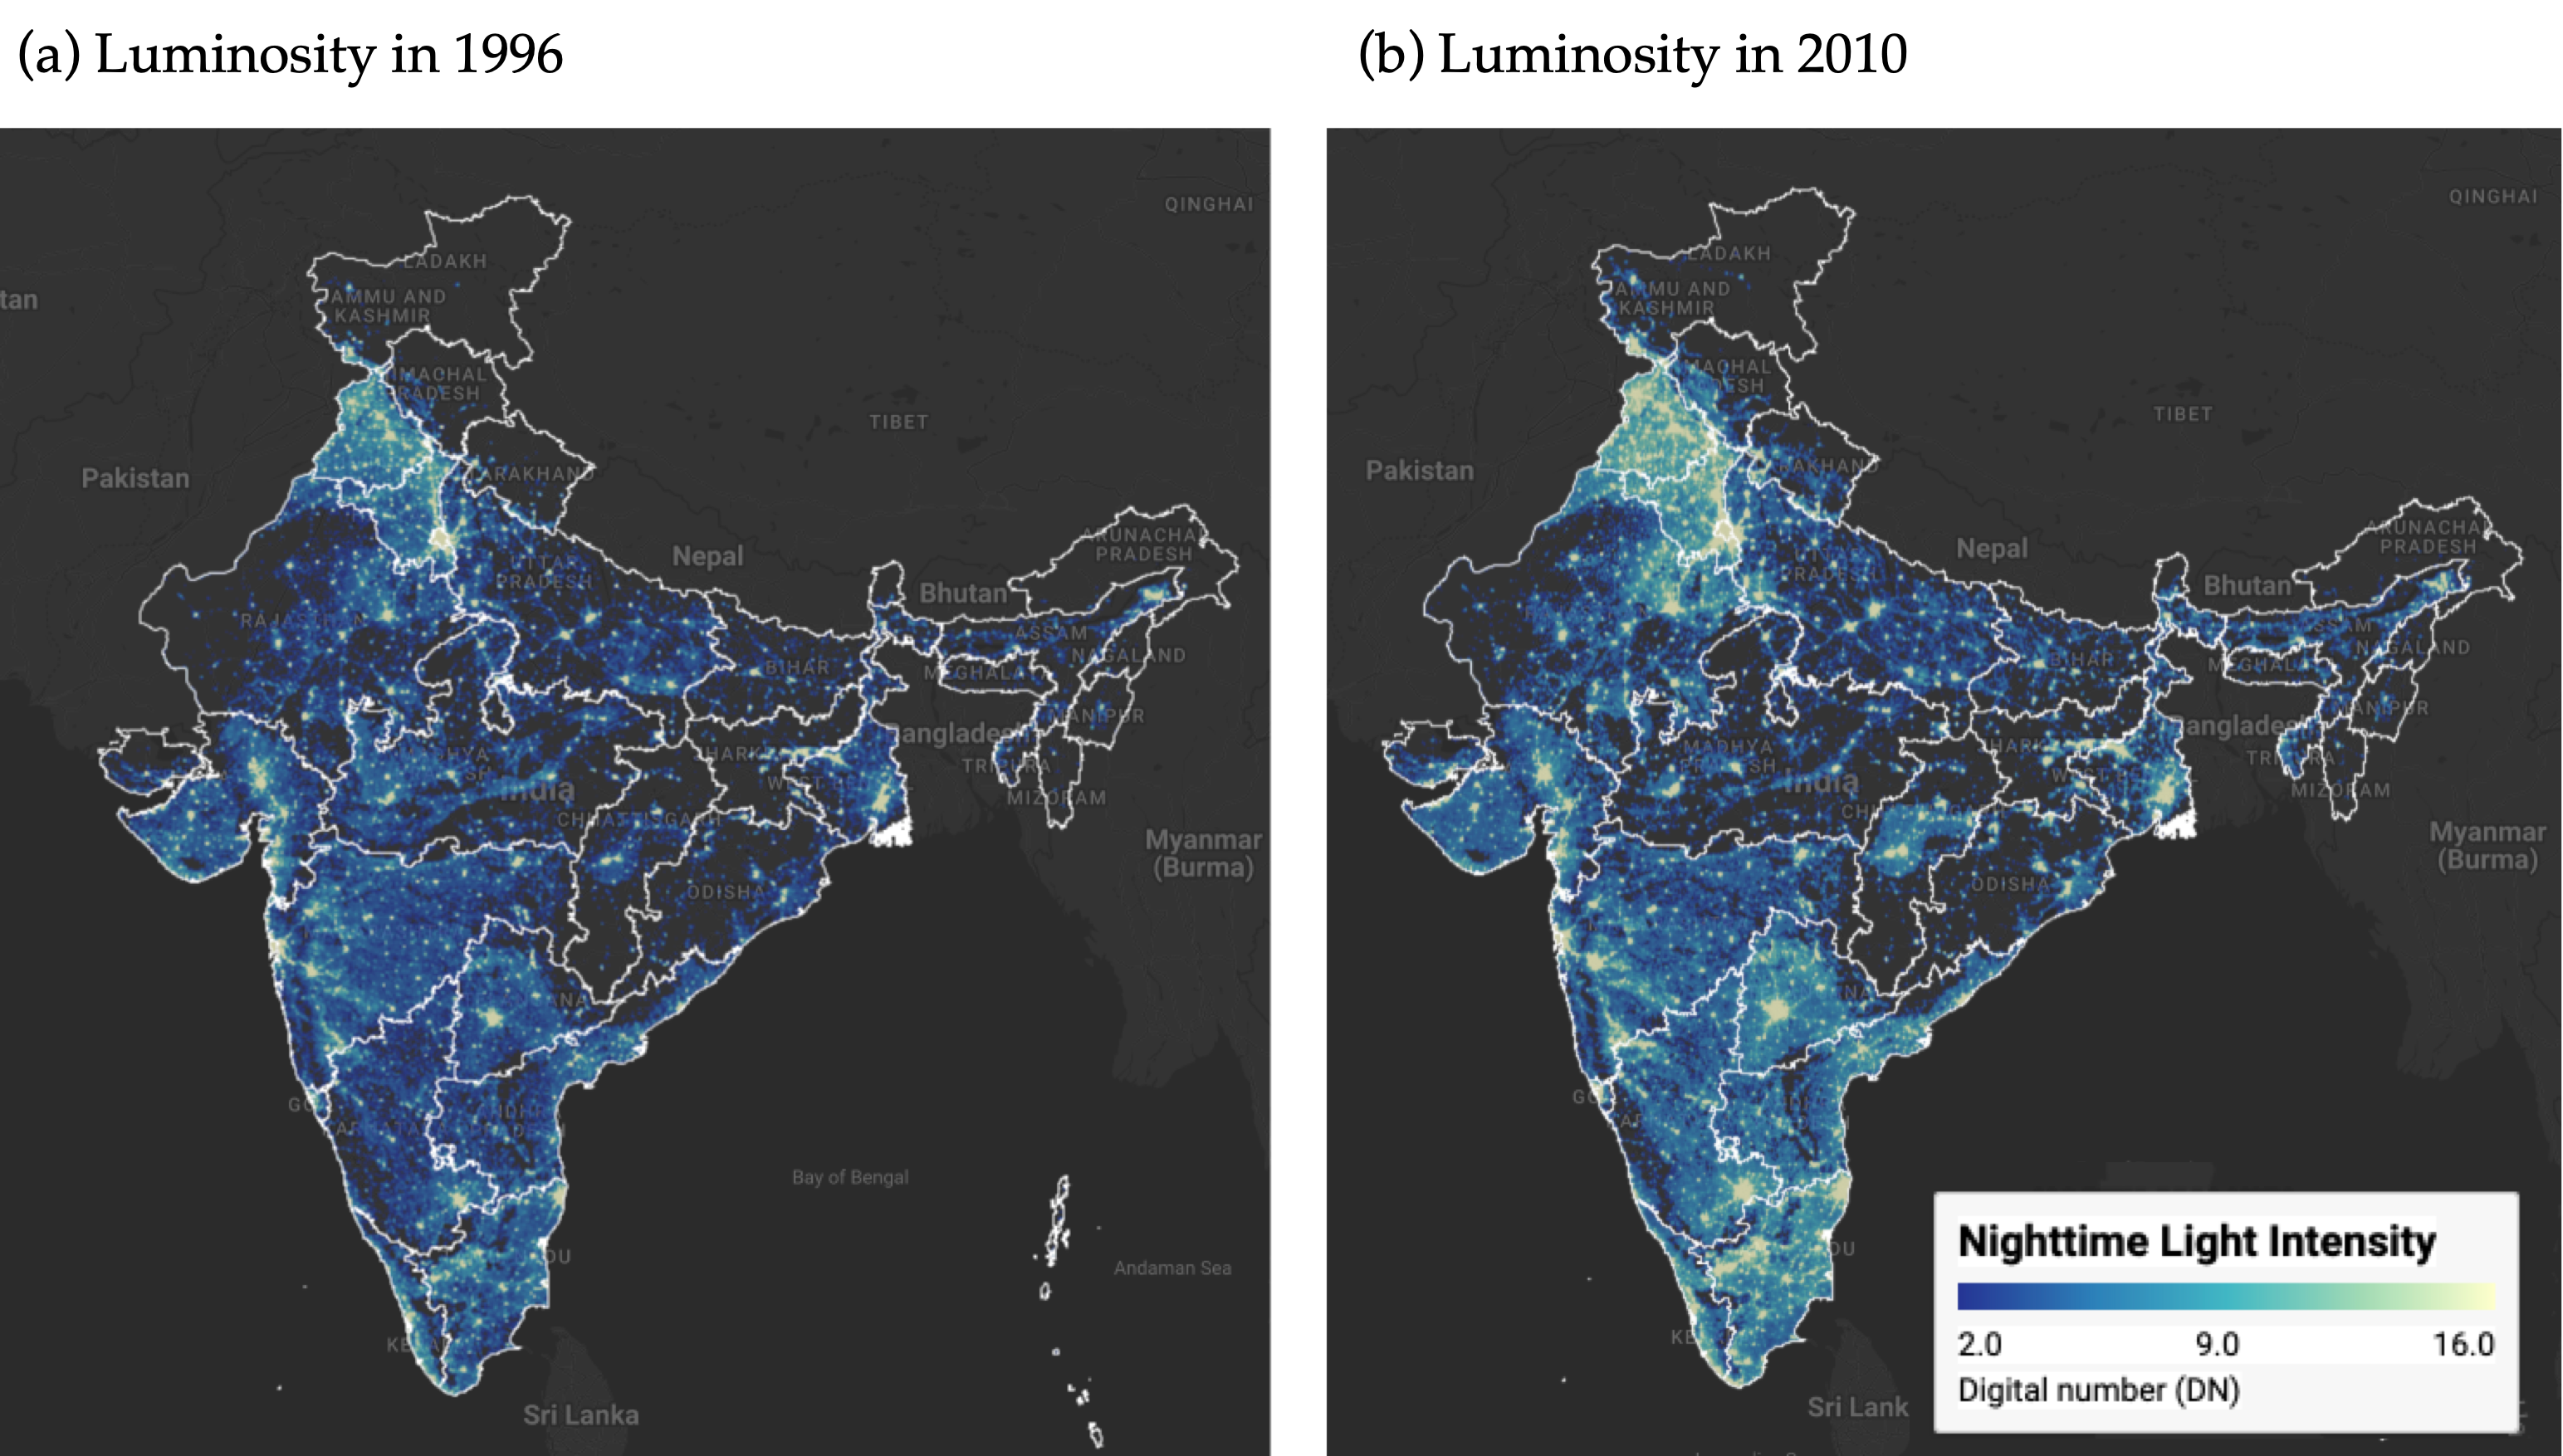
\includegraphics[keepaspectratio]{images/luminosity_map.png}}

}

\caption{\label{fig-map}Regional luminosity in India: 1996 vs 2010
Notes: Luminosity is measured in radiance-calibrated digital number (DN)
values from DMSP-OLS satellites. Interactive web application available
at \url{https://bit.ly/india-rc-ntl}. Source: Authors' visualization
using pre-processed luminosity images from the Earth Observation Group
(NOAA/NCEI). See
\href{https://quarcs-lab.github.io/project2025s-py/notebooks/c01_view_from_space.html}{View
from outer space} notebook for source code.}

\end{figure}%

Figure~\ref{fig-map} presents static maps of luminosity in the initial
and final years, 1996 and 2010, captured from our interactive
application. The maps show a noticeable increase in brightness across
most parts of India in 2010. Because nighttime lights serve as a proxy
for economic activity, this increase in luminosity reflects economic
growth over the period. Figure~\ref{fig-convergence} then illustrates
the relationship between per-capita growth in nighttime lights and
initial per-capita nighttime light. The scatterplot shows an inverse
relationship: the estimated \(\beta\)-convergence coefficient of about
\(-0.02\) implies an annual speed of convergence of roughly 2.3\% and a
half-life of about 30 years, consistent with the seminal finding of
Barro and Sala-i-Martin (1992). Because \(\beta\)-convergence need not
imply a narrowing of the distribution, we also check
\(\sigma\)-convergence: the cross-district standard deviation of log
per-capita luminosity falls from 1.09 in 1996 to 0.95 in 2010, a
reduction of 13.5\%, so spatial disparities did narrow over the period.

\begin{figure}[H]

\centering{

\pandocbounded{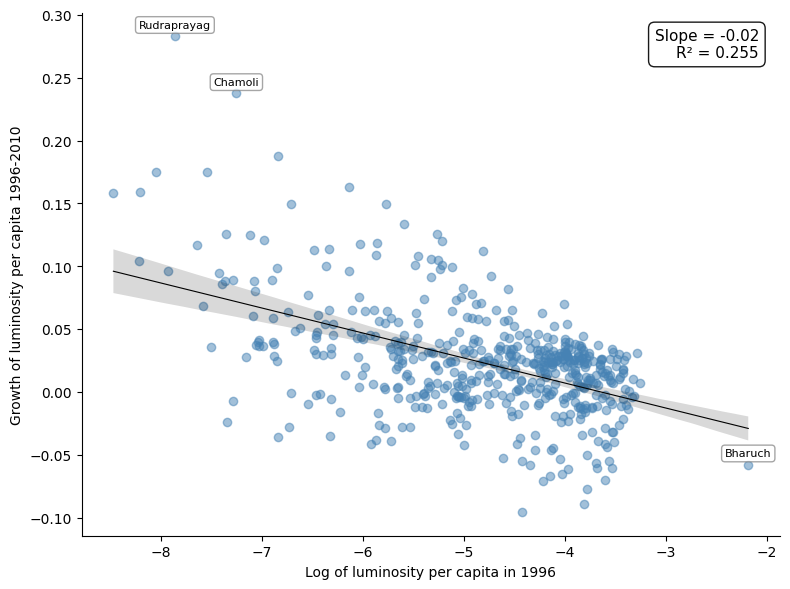
\includegraphics[keepaspectratio]{index_files/figure-latex/notebooks-c02_regional_convergence_sc-fig-convergence-output-1.png}}

}

\caption{\label{fig-convergence}Regional luminosity convergence across
districts in India Notes: Each point represents one of the 520
districts. The regression line shows the estimated beta-convergence
relationship. Outlier districts are labeled. Source: Data from Chanda
and Kabiraj (2020). See
\href{notebooks/c02_regional_convergence_sc.ipynb}{Regional convergence}
notebook for source code.}

\end{figure}%

Next, we examine case studies of three economically disadvantaged states
in India to illustrate their growth patterns over the study period.
Among these, Bihar is the poorest, with a per-capita income at 31.2\% of
the national average, while Uttar Pradesh and Chhattisgarh stand at
55.3\% and 59.9\% respectively.\footnote{The figures are relative per
  capita income for 2000--01, the census year closest to the start of
  our study period, measured as per capita net state domestic product
  divided by per capita net national income. They are taken from Table 4
  of Sanyal and Arora, ``Relative Economic Performance of Indian States:
  1960-61 to 2023-24'', Economic Advisory Council to the Prime Minister,
  Working Paper EAC-PM/WP/31/2024, September 2024.}
Figure~\ref{fig-map2} displays the change in luminosity in these three
states during our study period. Although these states remain among the
poorest, there is a noticeable increase in luminosity over the course of
the study.

\begin{figure}

\centering{

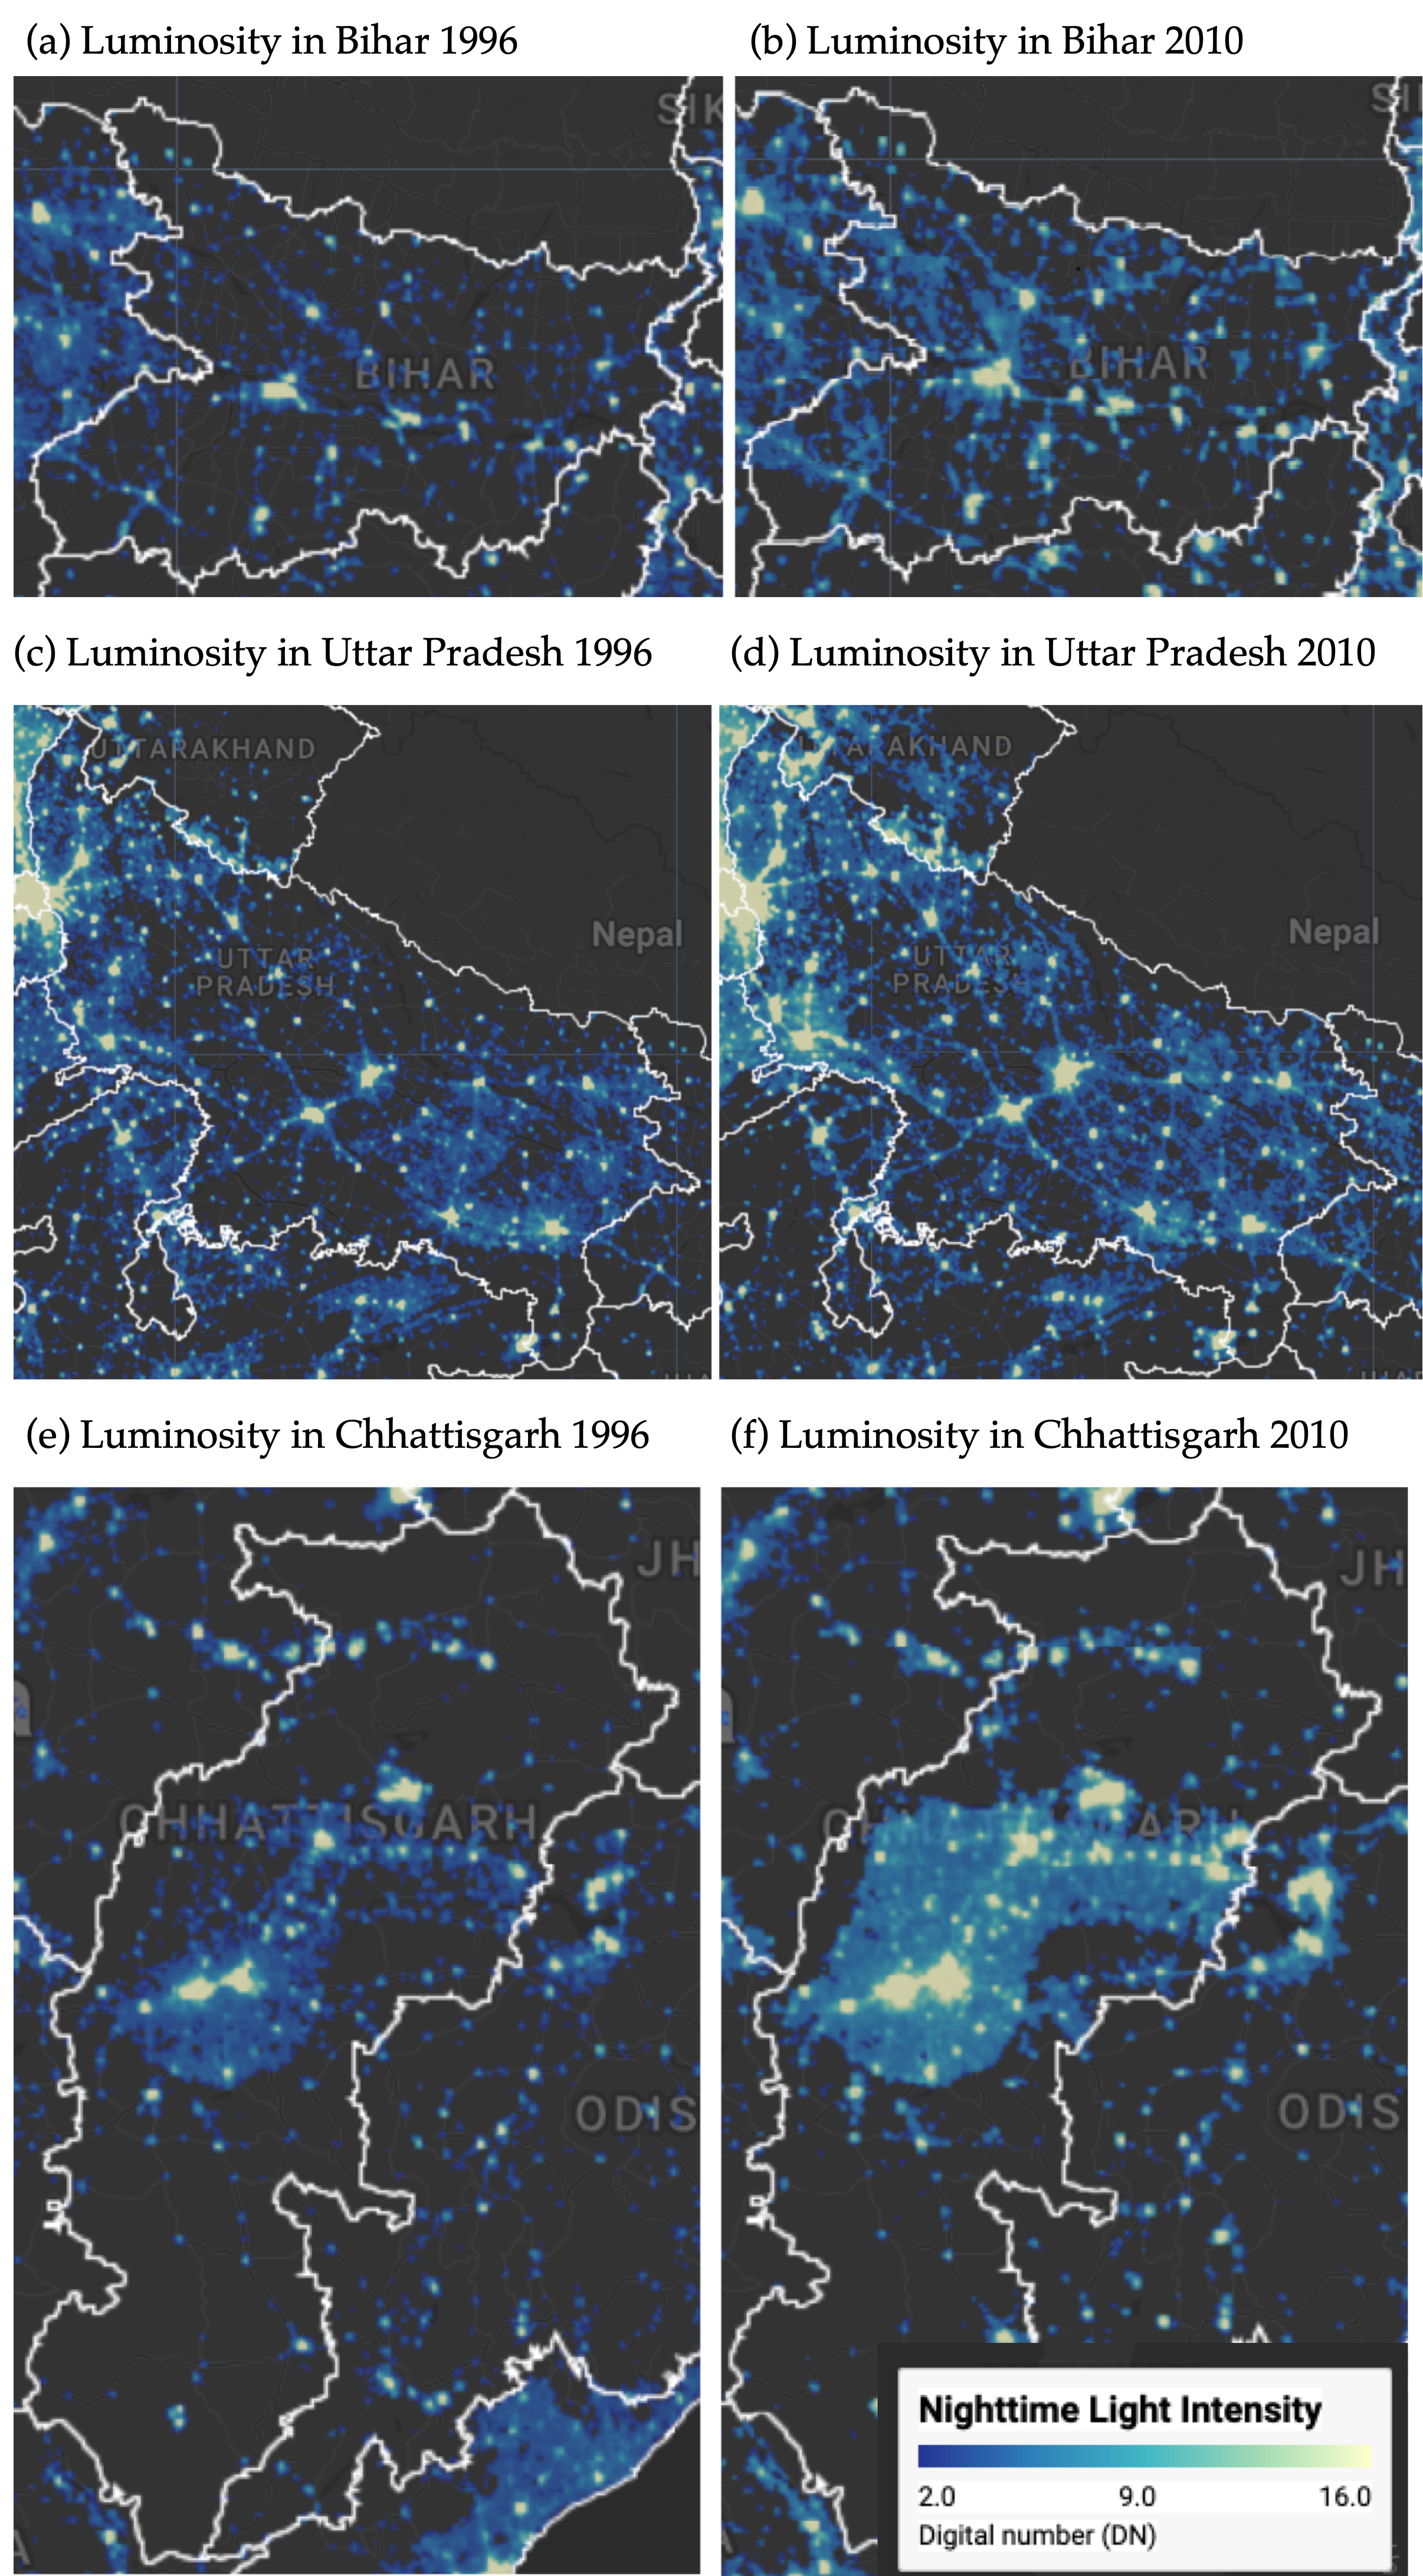
\includegraphics[width=0.75\linewidth,height=\textheight,keepaspectratio]{images/luminosity_map2.png}

}

\caption{\label{fig-map2}Some illustrative examples of regional
convergence Notes: Luminosity is measured in radiance-calibrated digital
number (DN) values from DMSP-OLS satellites. Interactive web application
available at \url{https://bit.ly/india-rc-ntl}. Source: Authors'
visualization using pre-processed luminosity images from the Earth
Observation Group (NOAA/NCEI). See
\href{https://quarcs-lab.github.io/project2025s-py/notebooks/c01_view_from_space.html}{View
from outer space} notebook for source code.}

\end{figure}%

\subsection{Spatial dependence is a feature of the convergence
process}\label{spatial-dependence-is-a-feature-of-the-convergence-process}

Before proceeding with the formal econometric analysis, we examine the
spatial distribution of the variables under study. Choropleth maps are a
natural tool for this purpose, because they show how a variable of
interest varies across geographic units and reveal patterns that summary
statistics alone would hide. Figure~\ref{fig-chorophleths} presents the
spatial distribution of initial luminosity in 1996 and of the subsequent
growth rate of luminosity over the 1996--2010 period across the 520
districts in our sample.

\begin{figure}[H]

\centering{

\pandocbounded{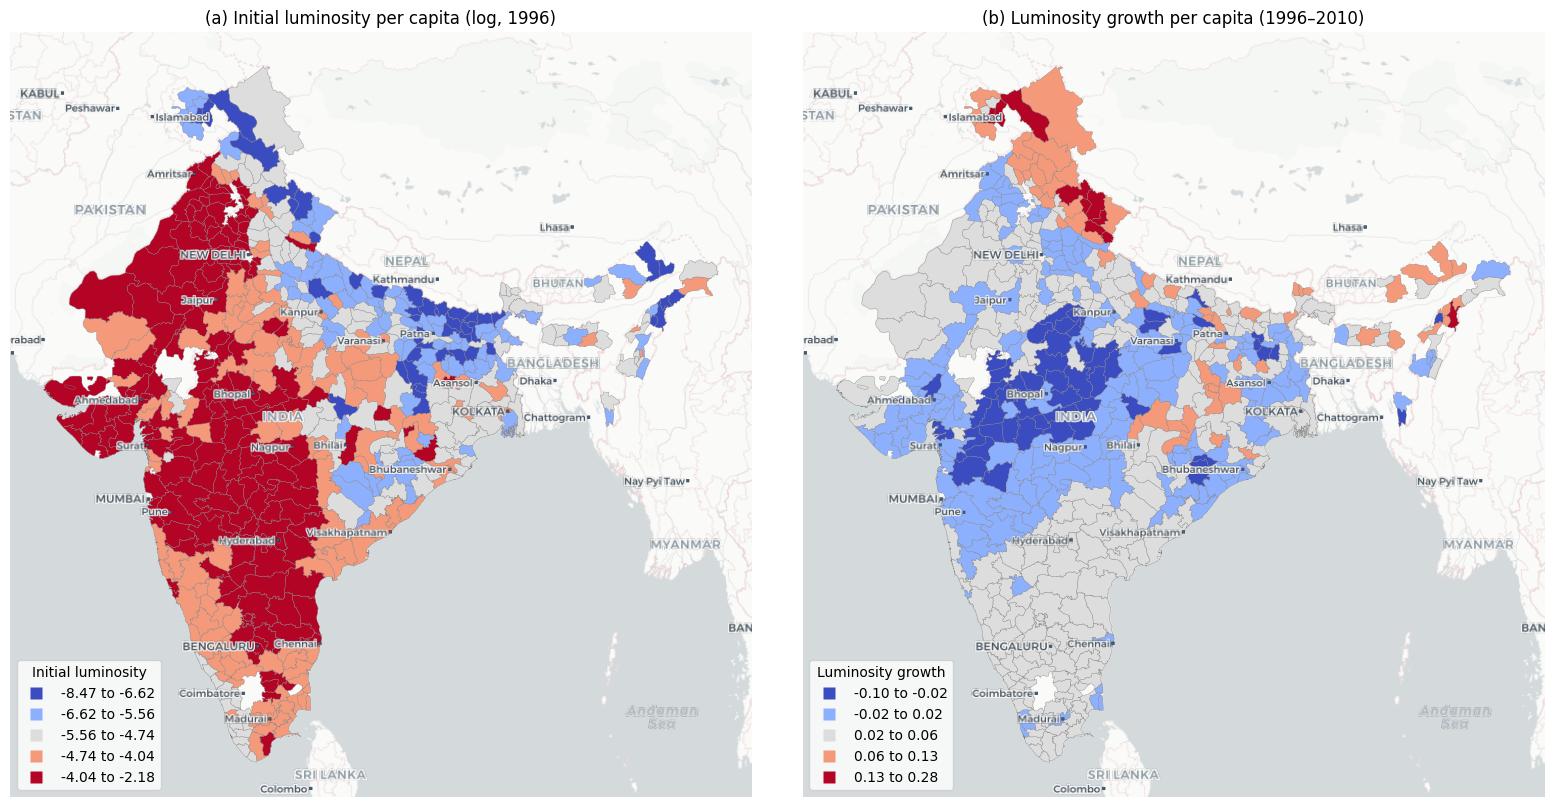
\includegraphics[keepaspectratio]{index_files/figure-latex/notebooks-c03_spatial_dependence_lisa-fig-chorophleths-output-1.png}}

}

\caption{\label{fig-chorophleths}Spatial distribution of initial
luminosity and luminosity growth Notes: Districts are classified into
five categories using Fisher-Jenks natural breaks. Panel (a) shows log
of luminosity per capita in 1996. Panel (b) shows luminosity growth per
capita over 1996--2010. Source: Data from Chanda and Kabiraj (2020). See
\href{notebooks/c03_spatial_dependence_lisa.ipynb}{Spatial dependence}
notebook for source code.}

\end{figure}%

The choropleth maps in Figure~\ref{fig-chorophleths} reveal a distinct
spatial pattern. Panel (a) shows that initial luminosity levels are
concentrated in specific geographic corridors, with higher values
clustered in western and north-western India, while large portions of
eastern and northern India exhibit markedly lower luminosity. Panel (b),
which displays the growth rate of luminosity per capita over the study
period, presents a pattern that is largely the inverse of the initial
distribution. Districts that were initially bright tend to exhibit lower
growth rates, whereas districts that were initially dim tend to grow at
a faster rate. This spatial inversion provides a first visual indication
that regional convergence in India may have an important spatial
dimension.

While the choropleth maps suggest the presence of spatial structure in
both variables, a formal analysis of spatial dependence requires a
definition of the neighborhood of each district. This neighborhood
structure is specified through a spatial weight matrix, which encodes
the connectivity between geographic units. In this study, we adopt a six
nearest neighbors weight matrix, so that for each of the 520 districts
the six nearest districts by centroid distance are identified as its
neighbors. This connectivity structure is visualized as a network in
Figure~\ref{fig-wmatrix6nn}, where each node represents a district
centroid and each edge connects a district to one of its six nearest
neighbors.

\begin{figure}[H]

\centering{

\pandocbounded{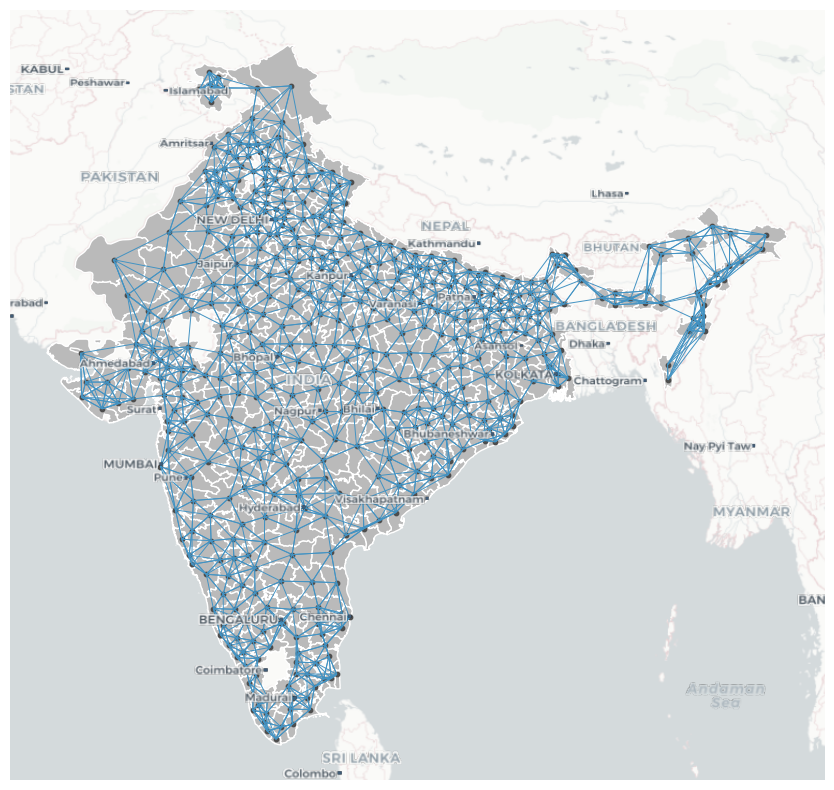
\includegraphics[keepaspectratio]{index_files/figure-latex/notebooks-c03_spatial_dependence_lisa-fig-wmatrix6nn-output-1.png}}

}

\caption{\label{fig-wmatrix6nn}Spatial connectivity structure based on
six nearest neighbors Notes: Each node represents a district centroid.
Each edge connects a district to one of its six geographically closest
neighbors. The weight matrix is row-standardized. Source: Data from
Chanda and Kabiraj (2020). See
\href{notebooks/c03_spatial_dependence_lisa.ipynb}{Spatial dependence}
notebook for source code.}

\end{figure}%

With the neighborhood of each district defined, we can formally assess
the degree of spatial dependence in the variables. Spatial dependence
can be understood through two complementary concepts: the overall degree
of clustering in the data, and the specific locations of statistically
significant clusters and spatial outliers. The Global Moran's I
statistic captures the first of these concepts. In our data, the Moran's
I for initial luminosity per capita is 0.73 (\(p = 0.001\)), which
indicates strong positive spatial autocorrelation: districts with high
(low) initial luminosity tend to be surrounded by districts that are
also bright (dim). The Moran's I for luminosity growth is 0.60
(\(p = 0.001\)), which confirms that the growth rates of neighboring
districts are also significantly correlated. Both the initial level and
the subsequent growth of luminosity therefore exhibit substantial
spatial clustering.

We now turn to the LISA statistics, which locate the significant
clusters and outliers behind these global measures.
Figure~\ref{fig-dependence-initial} presents the Moran scatterplot and
LISA cluster map for initial luminosity per capita. The cluster map
identifies distinct geographic concentrations. HH clusters mark the most
luminous regions and their bright neighbors, while LL clusters highlight
contiguous areas of low luminosity. These are predominantly in eastern
and northern India, in Bihar, eastern Uttar Pradesh, and Jharkhand,
together with the Himalayan north and the northeast.

\begin{figure}[H]

\centering{

\pandocbounded{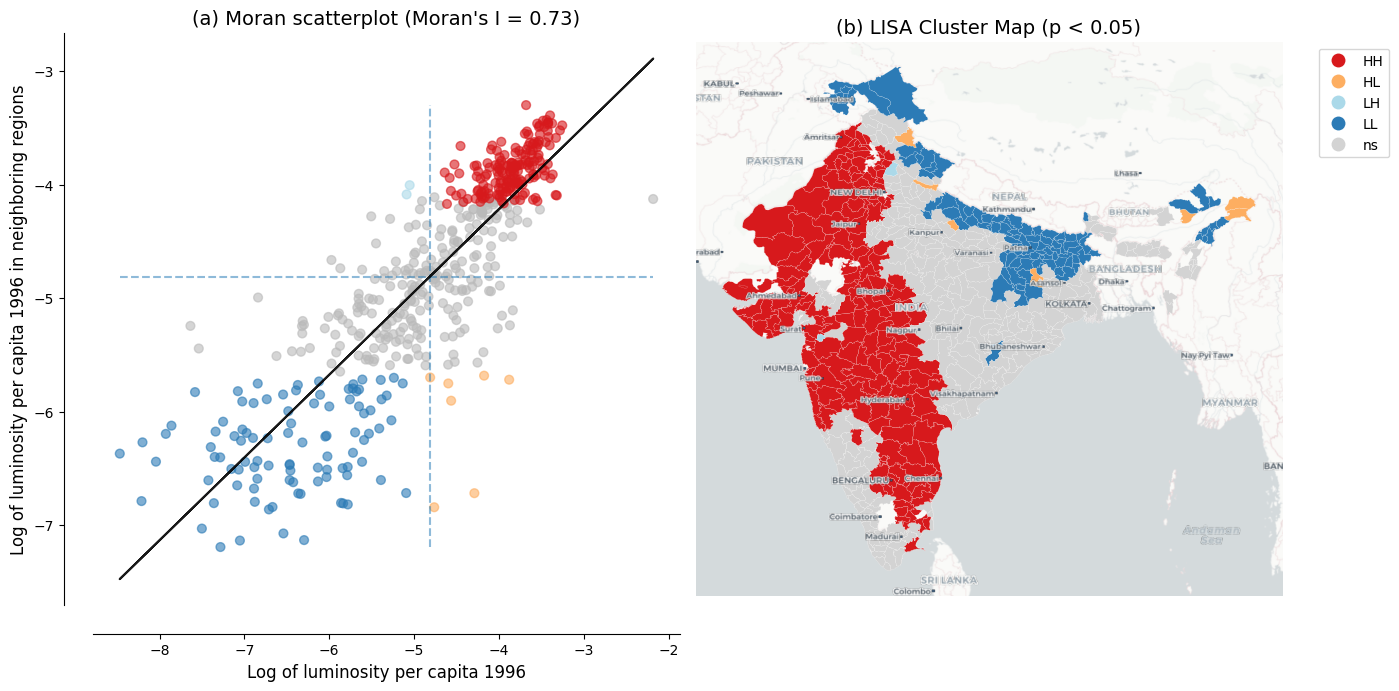
\includegraphics[keepaspectratio]{index_files/figure-latex/notebooks-c03_spatial_dependence_lisa-fig-dependence-initial-output-1.png}}

}

\caption{\label{fig-dependence-initial}Spatial dependence in the initial
level of luminosity Notes: Panel (a) shows the Moran scatterplot with
Global Moran's I statistic. Panel (b) shows the LISA cluster map with
statistically significant clusters at p \textless{} 0.05 based on 999
permutations. Source: Data from Chanda and Kabiraj (2020). See
\href{notebooks/c03_spatial_dependence_lisa.ipynb}{Spatial dependence}
notebook for source code.}

\end{figure}%

The same LISA analysis applied to luminosity growth rates reveals a
geographic pattern that is largely the inverse of the initial luminosity
clusters, as shown in Figure~\ref{fig-dependence-growth}. Districts that
formed HH clusters in initial luminosity tend to appear as LL clusters
in luminosity growth, and the dimmest clusters tend to emerge as HH
clusters in growth.\footnote{The initially prosperous areas therefore
  experienced relatively slower growth over the study period, while the
  initially lagging areas grew faster.} This spatial inversion between
the initial level and the subsequent growth of luminosity is the spatial
signature of the convergence process: red regions in the initial
luminosity map become blue regions in the growth map, and vice versa.
These local spatial patterns provide visual evidence that spatial
dependence is a prominent feature of the regional convergence process
observed in India, and they motivate the use of spatial econometric
methods.

\begin{figure}[H]

\centering{

\pandocbounded{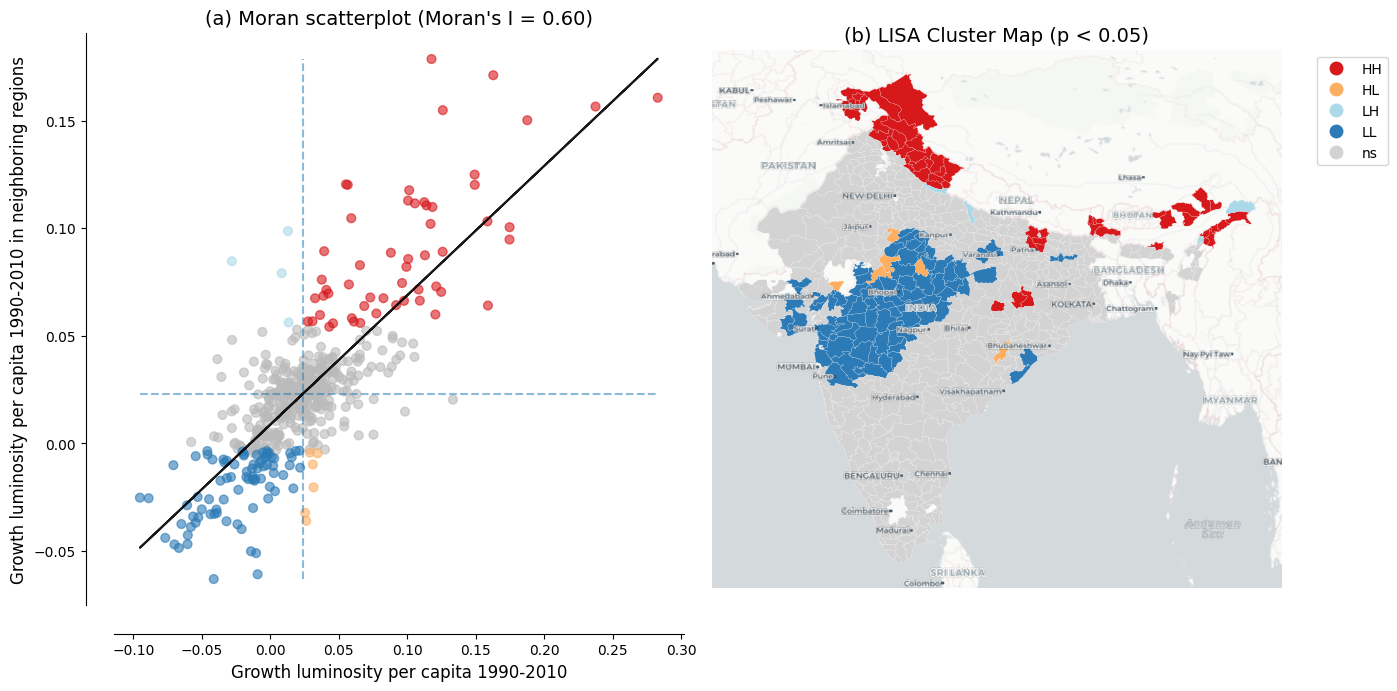
\includegraphics[keepaspectratio]{index_files/figure-latex/notebooks-c03_spatial_dependence_lisa-fig-dependence-growth-output-1.png}}

}

\caption{\label{fig-dependence-growth}Spatial dependence in the growth
rate of luminosity Notes: Panel (a) shows the Moran scatterplot with
Global Moran's I statistic. Panel (b) shows the LISA cluster map with
statistically significant clusters at p \textless{} 0.05 based on 999
permutations. Source: Data from Chanda and Kabiraj (2020). See
\href{notebooks/c03_spatial_dependence_lisa.ipynb}{Spatial dependence}
notebook for source code.}

\end{figure}%

\subsection{Evidence of spatial spillovers in regional
convergence}\label{evidence-of-spatial-spillovers-in-regional-convergence}

The regression results of Table~\ref{tbl-models} provide evidence of
both unconditional and conditional convergence across districts in
India. Both conventional ordinary least squares (OLS) and spatial
econometric approaches indicate significant negative relationships
between initial luminosity levels and subsequent growth rates. The
direct effects, which represent within-district convergence, remain
negative and of similar order across specifications, ranging from -0.020
to -0.026. This consistency across specifications and estimation methods
suggests that poorer districts are catching up to their wealthier
counterparts, even after controlling for district characteristics and
state-level fixed effects.

\begin{longtable}[]{@{}
  >{\raggedright\arraybackslash}p{(\linewidth - 16\tabcolsep) * \real{0.1282}}
  >{\raggedright\arraybackslash}p{(\linewidth - 16\tabcolsep) * \real{0.1154}}
  >{\raggedright\arraybackslash}p{(\linewidth - 16\tabcolsep) * \real{0.0897}}
  >{\raggedright\arraybackslash}p{(\linewidth - 16\tabcolsep) * \real{0.1154}}
  >{\raggedright\arraybackslash}p{(\linewidth - 16\tabcolsep) * \real{0.1154}}
  >{\raggedright\arraybackslash}p{(\linewidth - 16\tabcolsep) * \real{0.1154}}
  >{\raggedright\arraybackslash}p{(\linewidth - 16\tabcolsep) * \real{0.0897}}
  >{\raggedright\arraybackslash}p{(\linewidth - 16\tabcolsep) * \real{0.1154}}
  >{\raggedright\arraybackslash}p{(\linewidth - 16\tabcolsep) * \real{0.1154}}@{}}

\caption{\label{tbl-models}Unconditional and conditional convergence
across districts.}

\tabularnewline

\toprule\noalign{}
\begin{minipage}[b]{\linewidth}\raggedright
\end{minipage} & \begin{minipage}[b]{\linewidth}\raggedright
Model 1
\end{minipage} & \begin{minipage}[b]{\linewidth}\raggedright
\end{minipage} & \begin{minipage}[b]{\linewidth}\raggedright
Model 2
\end{minipage} & \begin{minipage}[b]{\linewidth}\raggedright
\end{minipage} & \begin{minipage}[b]{\linewidth}\raggedright
Model 3
\end{minipage} & \begin{minipage}[b]{\linewidth}\raggedright
\end{minipage} & \begin{minipage}[b]{\linewidth}\raggedright
Model 4
\end{minipage} & \begin{minipage}[b]{\linewidth}\raggedright
\end{minipage} \\
\midrule\noalign{}
\endhead
\bottomrule\noalign{}
\endlastfoot
& OLS & SDM & OLS & SDM & OLS & SDM & OLS & SDM \\
Direct & -0.020*** & -0.021*** & -0.022*** & -0.021*** & -0.025*** &
-0.026*** & -0.025*** & -0.025*** \\
& (0.002) & (0.002) & (0.003) & (0.002) & (0.003) & (0.002) & (0.003) &
(0.002) \\
Indirect & -- & -0.001 & -- & -0.001 & -- & -0.015* & -- & -0.012* \\
& & (0.006) & & (0.005) & & (0.008) & & (0.007) \\
Total & -0.020*** & -0.022*** & -0.022*** & -0.022*** & -0.025*** &
-0.041*** & -0.025*** & -0.037*** \\
& (0.002) & (0.006) & (0.003) & (0.005) & (0.003) & (0.009) & (0.003) &
(0.007) \\
Controls & No & No & No & No & Yes & Yes & Yes & Yes \\
State FE & No & No & Yes & Yes & No & No & Yes & Yes \\
AIC & -1945 & -2292 & -2409 & -2468 & -2211 & -2358 & -2465 & -2501 \\

\end{longtable}

The progression from unconditional to conditional specifications reveals
how the estimated convergence process is shaped by the inclusion of
additional covariates. In the OLS specifications, the direct effect is
-0.020 in Model 1 and -0.022 in Model 2, and it strengthens to -0.025
once district characteristics are added in Models 3 and 4. Omitting
these characteristics therefore attenuates the estimated speed of
convergence. The spatial Durbin direct effects match this pattern in the
conditional models, at -0.026 in Model 3 and -0.025 in Model 4. Once we
account for structural differences across districts, the underlying
tendency for poorer districts to catch up becomes more pronounced. State
fixed effects absorb unobserved state-level heterogeneity, such as
differences in governance and institutional quality, that might
otherwise confound the convergence relationship. They tighten the
standard errors on the spatial impacts and moderate the spatial total
effect rather than strengthening it further.

The spatial Durbin model also reveals spatial spillover effects that are
not captured by traditional OLS estimations. These indirect effects,
which capture the influence of the initial conditions of neighboring
districts on the growth rate of a district, follow a notable pattern
across specifications. In the unconditional models (Models 1 and 2), the
estimated indirect effects are negative but small and statistically
insignificant, at -0.001 in both.\footnote{Without controls, the strong
  residual spatial dependence confounds the spillover estimates with
  omitted variables. The spatial autoregressive parameter also reaches
  about 0.80 in Model 1, so its decomposition is the most sensitive of
  the four to how the spatial multiplier is computed.} Once
district-level controls are introduced (Models 3 and 4), the indirect
effects become both larger in magnitude and statistically significant at
the 10\% level, reaching -0.015 in Model 3 and -0.012 in our most
comprehensive Model 4. The spatial channels of convergence therefore
become discernible only after accounting for district-specific
characteristics.

The total impact of initial conditions on growth, combining both direct
and spillover effects, is substantially larger when we account for
spatial dependence. In our fully specified model (Model 4), the total
convergence effect in the spatial Durbin model (-0.037) is approximately
51\% larger in magnitude than the OLS estimate (-0.025). Translated into
an annual speed of convergence, this raises the implied speed from about
3.0\% under OLS to about 5.2\% under the SDM, and it shortens the
implied half-life from roughly 23 to 13 years. The gap is even larger in
Model 3 (SDM total -0.041 against OLS -0.025, or 67\%), but the Model 3
and Model 4 spillover estimates are statistically indistinguishable, so
we anchor our interpretation on the preferred Model 4. These differences
indicate that in this setting conventional non-spatial approaches
understate the speed of regional convergence by failing to capture the
additional convergence channels created through spatial spillovers.

\begin{longtable}[]{@{}lllll@{}}

\caption{\label{tbl-speed}Implied annual speed of convergence and
half-life by model, from the OLS and SDM total effects of initial
luminosity.}

\tabularnewline

\toprule\noalign{}
Model & OLS speed & SDM speed & OLS half-life & SDM half-life \\
\midrule\noalign{}
\endhead
\bottomrule\noalign{}
\endlastfoot
Model 1 & 2.3\% & 2.6\% & 30 yr & 27 yr \\
Model 2 & 2.6\% & 2.7\% & 27 yr & 26 yr \\
Model 3 & 3.0\% & 6.2\% & 23 yr & 11 yr \\
Model 4 & 3.0\% & 5.2\% & 23 yr & 13 yr \\

\end{longtable}

Table~\ref{tbl-speed} reports the implied speeds and half-lives for all
four specifications. The spatial premium is concentrated in the
conditional models. In Models 1 and 2 the OLS and SDM speeds are nearly
identical, whereas in Models 3 and 4 the SDM raises the implied speed
from 3.0\% to 6.2\% and 5.2\%, shortening the half-life from 23 years to
11 and 13 years respectively.\footnote{The unconditional speeds are
  2.3\% against 2.6\% in Model 1 and 2.6\% against 2.7\% in Model 2.}

The model fit statistics further support the spatial econometric
approach. The Akaike Information Criterion (AIC) consistently favors the
spatial Durbin model over OLS across all four specifications, and the
most comprehensive model (Model 4 SDM) achieves the lowest AIC value of
-2501 compared to -2465 for the corresponding OLS.\footnote{The
  improvement from incorporating spatial structure is most pronounced in
  the unconditional specification, where the AIC drops by 347 units when
  moving from OLS to SDM in Model 1, reflecting the large amount of
  spatial dependence left unmodeled by ordinary regressions. Even in the
  fully specified model, where state fixed effects already absorb much
  of the spatial heterogeneity, the SDM retains a meaningful advantage.}
Overall, these results suggest that regional convergence in India
operates not only through district-specific factors but also through
spatial interactions between neighboring districts. In this setting,
ignoring these interactions leads to both underestimated convergence
speeds and inferior model performance.

A word of caution is in order about how the indirect effects should be
read. The spatial Durbin model identifies spatial dependence in reduced
form: it establishes that the growth of a district covaries with the
initial conditions of its neighbors, conditional on its own
characteristics, but it does not establish why. Several distinct
processes generate the same reduced-form pattern. Neighboring districts
share geographic and agro-climatic conditions. They are often governed
by the same state, and so inherit common institutional and policy
environments that our state fixed effects absorb only in part. They are
connected by infrastructure whose effects do not stop at administrative
boundaries. Any omitted determinant of growth that is itself spatially
clustered will also be absorbed into the spatial terms of the model. The
measurement issues discussed below point in the same direction, since
blooming spreads light across district boundaries and can raise the
apparent correlation between neighbors for reasons unrelated to economic
interaction. We therefore read the indirect effects as evidence that
spatial structure is a feature of the convergence process, and not as an
estimate of the causal effect of the conditions of one district on the
growth of another. Establishing which channels are at work, and whether
they are causal, would require research designs built for that purpose,
a point we return to in the discussion.

\subsection{How these estimates compare with the convergence
literature}\label{how-these-estimates-compare-with-the-convergence-literature}

The speeds reported above can be placed against three sets of
benchmarks. The first is other work on Indian districts using the same
proxy: Beyer and Yamada (2020) report 2.4\% absolute and 3.7\%
conditional convergence for India over 2013--2019, against our own 2.3\%
and 3.0\%. That two independent applications of the same measurement
strategy recover similar non-spatial rates, despite different periods
and different generations of the sensor, is reassuring about the proxy.

The second comparison is with convergence estimated from luminosity
elsewhere. Basher, Rashid, and Uddin (2023) find 4.57\% per year across
the 64 districts of Bangladesh, implying a half-life of 15 years, above
the 2.3\% we obtain without controls and below the 5.2\% of our
preferred spatial model. Carrington and Jiménez-Ayora (2021) report a
speed near the 2\% benchmark for Ecuadorian provinces, while Kacou
(2022) finds multiple equilibria in within-country regional inequality
across 49 African countries. Our unconditional non-spatial estimate
therefore sits near the familiar 2\% regularity, and the conditional
spatial estimates well above it.\footnote{The regularity is about 2\%
  per year across 1,528 regions in 83 countries (Gennaioli et al. 2014),
  and similar across regions of the United States, Japan, and five
  European countries (Sala-i-Martin 1996).} That regularity should not
be treated as a law: a meta-analysis of some 600 published estimates
concludes that it is misleading to speak of a natural convergence rate,
since estimates from different specifications are drawn from different
populations (Abreu, de Groot, and Florax 2005). These comparisons
therefore locate our estimates rather than validate them.

The third comparison bears most directly on what this article adds. That
convergence estimates are sensitive to spatial dependence is
established; the direction in which allowing for it moves the estimated
speed is not. Our own rise from 3.0\% to 5.2\% agrees with Diop (2018),
who finds a substantially higher speed in a spatial Durbin specification
and concludes that earlier estimates may have been considerably
understated. Other studies find the opposite. Isla-Castillo, Garashchuk,
and Podadera-Rivera (2024) report lower estimated speeds for European
regions once spatial dependence is allowed for, and Santos-Marquez,
Gunawan, and Mendez (2022) conclude that neighbor effects have slowed
convergence across Indonesian districts. Within India, Lolayekar and
Mukhopadhyay (2019) find a considerably smaller impact of initial income
across states, and divergence rather than convergence.

The arithmetic is straightforward in our own case: the indirect effect
carries the same negative sign as the direct effect, so the two
reinforce one another and the total effect exceeds the OLS coefficient
in magnitude. Where the initial conditions of neighbors enter with the
opposite sign, or where the spatial terms absorb variation the
non-spatial model had attributed to initial luminosity, the same
exercise reduces the estimated speed. The substantive point is therefore
not that spatial dependence matters, which is already known, but that
here it works in the direction of faster measured convergence, and the
contrast with Indian states suggests that the scale of analysis is part
of what determines the answer.

\subsection{Robustness to alternative spatial weight
matrices}\label{robustness-to-alternative-spatial-weight-matrices}

The spillover results above use a six-nearest-neighbor (6NN) spatial
weight matrix. To assess their sensitivity to this choice, we
re-estimate the preferred Model 4 under six alternative specifications
and compare them with the 6NN baseline. The alternatives are four- and
eight-nearest neighbors, queen and rook contiguity, and inverse distance
and inverse-distance-squared, the last two applied within a distance
band.

\begin{figure}[H]

\centering{

\pandocbounded{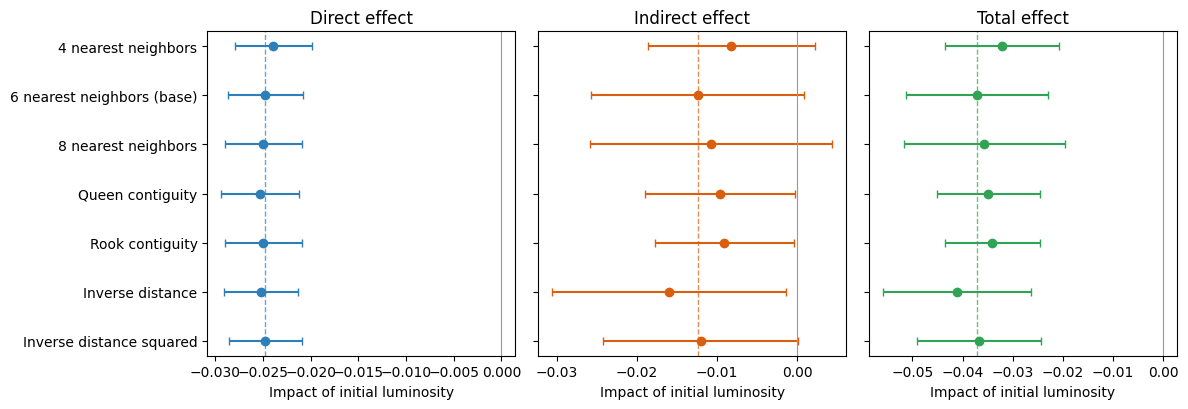
\includegraphics[keepaspectratio]{index_files/figure-latex/notebooks-c07_alternative_w_matrices-fig-altw-output-1.png}}

}

\caption{\label{fig-altw}Robustness of the Model 4 spatial impacts of
initial luminosity to the choice of spatial weight matrix. Points are
Direct, Indirect, and Total impacts; bars are 95\% Monte-Carlo
confidence intervals. The dashed lines mark the 6NN baseline estimates.}

\end{figure}%

\begin{longtable}[]{@{}
  >{\raggedright\arraybackslash}p{(\linewidth - 8\tabcolsep) * \real{0.3333}}
  >{\raggedright\arraybackslash}p{(\linewidth - 8\tabcolsep) * \real{0.1778}}
  >{\raggedright\arraybackslash}p{(\linewidth - 8\tabcolsep) * \real{0.2222}}
  >{\raggedright\arraybackslash}p{(\linewidth - 8\tabcolsep) * \real{0.1556}}
  >{\raggedright\arraybackslash}p{(\linewidth - 8\tabcolsep) * \real{0.1111}}@{}}

\caption{\label{tbl-altw}Model 4 spatial impacts of initial luminosity
under alternative spatial weight matrices (full LeSage--Pace method;
Monte-Carlo standard errors in parentheses).}

\tabularnewline

\toprule\noalign{}
\begin{minipage}[b]{\linewidth}\raggedright
Weight matrix
\end{minipage} & \begin{minipage}[b]{\linewidth}\raggedright
Direct
\end{minipage} & \begin{minipage}[b]{\linewidth}\raggedright
Indirect
\end{minipage} & \begin{minipage}[b]{\linewidth}\raggedright
Total
\end{minipage} & \begin{minipage}[b]{\linewidth}\raggedright
AIC
\end{minipage} \\
\midrule\noalign{}
\endhead
\bottomrule\noalign{}
\endlastfoot
4 nearest neighbors & -0.024***(0.002) & -0.008(0.005) &
-0.032***(0.006) & -2468 \\
6 nearest neighbors (base) & -0.025***(0.002) & -0.012*(0.007) &
-0.037***(0.007) & -2501 \\
8 nearest neighbors & -0.025***(0.002) & -0.011(0.008) &
-0.036***(0.008) & -2485 \\
Queen contiguity & -0.025***(0.002) & -0.010**(0.005) & -0.035***(0.005)
& -2463 \\
Rook contiguity & -0.025***(0.002) & -0.009**(0.004) & -0.034***(0.005)
& -2469 \\
Inverse distance & -0.025***(0.002) & -0.016**(0.007) & -0.041***(0.008)
& -2486 \\
Inverse distance squared & -0.025***(0.002) & -0.012*(0.006) &
-0.037***(0.006) & -2485 \\

\end{longtable}

The direct and total convergence effects are robust to the choice of
spatial weights, and the spillover component is consistently negative
but more sensitive (Figure~\ref{fig-altw} and Table~\ref{tbl-altw}). The
direct (within-district) convergence effect is essentially unchanged
across all seven specifications, ranging from -0.024 to -0.025 and
always significant at the 1\% level. The total convergence effect
likewise remains negative and significant throughout, ranging from
-0.032 to -0.041, with the 6NN baseline (-0.037) near the middle of this
range. The indirect (spillover) component is negative in every
specification and statistically significant under five of the seven,
which is a consistent if weaker pattern. This stability indicates that
the direct and total convergence effects are not an artifact of the
particular neighbor definition.

The results reported so far treat luminosity as a proxy for economic
output, which is the use that the convergence literature has made of it.
The discussion that follows asks first what the magnitude of these
estimates implies for regional policy, and what rests on the use of a
single growth period. It then turns to a second use of the same data,
since nighttime lights also record electrification, urbanization, and
broader socioeconomic conditions, and the reproducible workflow
assembled here can be pointed at those dimensions as readily as at
output. That possibility is pursued in an exploratory way, asking how
luminosity relates to cultural participation across Indian states.

\section{Discussion}\label{discussion}

\subsection{What the magnitude of the effects implies for regional
policy}\label{what-the-magnitude-of-the-effects-implies-for-regional-policy}

The difference between the two readings of Model 4 is large enough to
matter for policy. Under the OLS estimate, a district closes half of the
gap to its steady state in about 23 years; under the spatial Durbin
estimate, in about 13 years. Over the fourteen years of our sample, that
is the difference between closing roughly 34\% of the initial gap and
closing roughly 52\% of it. The first figure describes catch-up over a
generation, while the second describes catch-up within the horizon over
which development programs are designed, funded, and evaluated.

The distinction matters because it changes what can reasonably be
expected of an intervention. If convergence is slow, support for lagging
districts must be sustained across political cycles before its effects
become visible in aggregate outcomes, and the absence of visible
catch-up within the lifetime of a program is weak evidence that the
program has failed. If convergence is faster, as the spatial estimates
imply, the returns to a well-targeted intervention should appear within
a normal evaluation window, and the case for measuring them is
correspondingly stronger.

The results also speak to the level at which such policies should
operate. We find convergence across districts over 1996--2010, whereas
Lolayekar and Mukhopadhyay (2019), working with Indian states over a
longer period, find divergence. Catch-up that is visible at the district
level and absent at the state level is consistent with the district
being the more informative unit of intervention, as the Aspirational
Districts Programme of India already assumes, although the two studies
also differ in outcome variable and period.\footnote{The programme was
  launched in 2018 to direct additional resources to the least developed
  districts of the country.} The spatial results add a qualification to
that logic: the growth of a district is associated with the initial
conditions of its neighbors, so a lagging district surrounded by other
lagging districts is in a different position from one adjacent to a
growing cluster, and a targeting rule that ranks districts one at a time
will not register that difference.

Spillovers, however, cut both ways, and the Indian evidence on
place-based policy is a caution as much as an encouragement. Hasan,
Jiang, and Rafols (2021) evaluate a tax-exemption program for
industrially backward districts and find that the resulting increase in
firm entry and employment was driven in part by the displacement of
activity from neighboring districts that narrowly missed qualifying, and
that the effects did not persist once the program ended. Activity moved
across a boundary would appear in our framework as a spatial
relationship between neighbors, and it is not the kind of spillover on
which a case for coordinated regional policy can be built. What the
satellite record does support is measurement: luminosity is responsive
enough to register a place-based package at this scale.\footnote{Shenoy
  (2018) uses nighttime lights to evaluate a large place-based package
  in Uttarakhand and finds that luminosity rises sharply on the targeted
  side of the new state border, which shows that the outcome we study is
  responsive enough to register policy at this scale.}

These implications follow if the indirect effects reflect genuine
interaction between districts. As set out in the results, the
reduced-form evidence is consistent with that reading but does not
establish it. The policy conclusions above should therefore be read with
that qualification attached.

\subsection{The single growth period and what a panel would
require}\label{the-single-growth-period-and-what-a-panel-would-require}

The estimates reported above rest on a single growth period, and the
cost of that design should be stated plainly. One long difference cannot
trace how the rate of convergence evolved within the period. It cannot
establish whether the spatial spillovers were stronger in some years
than in others, or whether they emerged only part-way through. It also
cannot separate long-run convergence from whatever was specific to these
fourteen years, which in India included the maturing of the post-1991
reforms.

These limitations are real, and the dynamics they concern matter, but
examining those dynamics lies beyond the scope of an article that adds a
spatial dimension to an existing cross-sectional result rather than
replacing it with a dynamic one. The immediate obstacle is the data: the
dataset we adopt from Chanda and Kabiraj (2020) holds
radiance-calibrated luminosity at six dates between 1996 and 2010, but
district population is observed only at the decennial censuses, so
per-capita luminosity at the intermediate dates would rest on
interpolated denominators. Over a single long difference that
interpolation touches only the endpoints, whereas in a panel it would
enter every observation, and in the time dimension that a panel exists
to exploit.

The more interesting question is what such a panel would be worth, and
here two distinct problems compound. The first belongs to growth
econometrics and predates nighttime lights: panel estimates of
convergence run far above cross-sectional ones, and Caselli, Esquivel,
and Lefort (1996) obtain a rate near 10\% per year using panel methods
that instrument for endogenous regressors, against the 2\% that
cross-sections deliver.\footnote{Barro (2015) argues that country fixed
  effects generate a misleadingly high convergence rate, and that
  combining post-1960 with post-1870 evidence returns a figure close to
  the conventional 2\%. Meta-analytic evidence finds that corrections
  for unobserved heterogeneity raise estimated convergence
  systematically (Abreu, de Groot, and Florax 2005).} How that gap
should be read remains contested, so a panel would not give a
better-identified version of our estimate but an estimate of something
different, whose relation to the long-run rate is itself disputed.

The second problem is specific to the proxy: luminosity discriminates
differences across places considerably better than changes over time (X.
Chen and Nordhaus 2019; Asher et al. 2021). Convergence, however, is a
long-run process, so the horizon over which it is measured determines
whether lights carry the relevant signal at all. Over fourteen years
most identifying variation is cross-sectional, which is what lights
currently support best; over the annual intervals that make panel
methods attractive the ratio of signal to measurement error falls
sharply. A short-horizon panel would therefore pair a specification that
is hard to interpret with a proxy operating where it is weakest.
Chakrabarty and Mukherjee (2022) estimate district convergence across
the pandemic period, and how such estimates should be read depends on
how much of the short-run movement in lights reflects output rather than
measurement.

Our own view follows from this. If panel methods are to be applied to
convergence in luminosity, the periods compared should be long, a
sequence of non-overlapping long differences rather than a
high-frequency panel. Harmonized DMSP--VIIRS series now make that
feasible across roughly three decades (Li et al. 2020), and
re-estimating this specification in that form is the most promising
temporal extension of the work reported here.

\subsection{An exploratory extension: Luminosity and cultural
participation}\label{an-exploratory-extension-luminosity-and-cultural-participation}

Nighttime lights capture not just GDP but a composite of
electrification, urbanization, infrastructure, and broader socioeconomic
conditions (Henderson, Storeygard, and Weil 2012; Mellander et al.
2015). In this section, we examine the association between luminosity
and cultural participation patterns across Indian states.

A growing literature argues that regional cultural attitudes constitute
an independent factor in economic development, not merely a by-product
of income or institutions. In particular, Tubadji (2025) applies the
Culture-Based Development framework, whose central claim is a
directional one. Cultural attitudes and the participation patterns that
reveal them are treated as a factor shaping local development, rather
than as an outcome that development produces. That direction also marks
the limit of what the exercise below can establish.\footnote{A
  cross-sectional association is consistent with either direction, and
  with both operating at once. What it can do is establish that the two
  are related, and describe the form that relationship takes.}

For India, the National Sample Survey (NSS) 47th Round (July--December
1991) surveys household cultural participation. Following the
Culture-Based Development framework, we reduce these survey items to six
dimensions and aggregate them to state means.\footnote{The six
  dimensions are live cultural performance, cultural telecast
  (TV/media), socio-cultural participation, cultural heritage and
  religion, live cultural shows, and sports. They are extracted from the
  survey items by principal-components analysis. See the
  \href{https://quarcs-lab.github.io/project2025s-py/notebooks/c06_spatial_culture.html}{Spatial
  culture} notebook for details and extended analyses.} With nighttime
lights data for an adjacent period (1992) now available for 32 Indian
states and union territories, we can examine the extent to which
luminosity is associated with regional cultural patterns. This part of
the analysis uses the Consistent and Corrected Nighttime Lights series
rather than the radiance-calibrated composites used above, because it is
the product that covers 1992. Given the small sample size (N = 32) and
the potential leverage of small territories at the extremes of the
distribution on linear correlation measures, we report Spearman rank
correlations throughout this section. Figure~\ref{fig-culture-scatter}
presents the relationship between log nighttime lights per capita and
the two cultural dimensions that show statistically significant
associations.

\begin{figure}[H]

\centering{

\pandocbounded{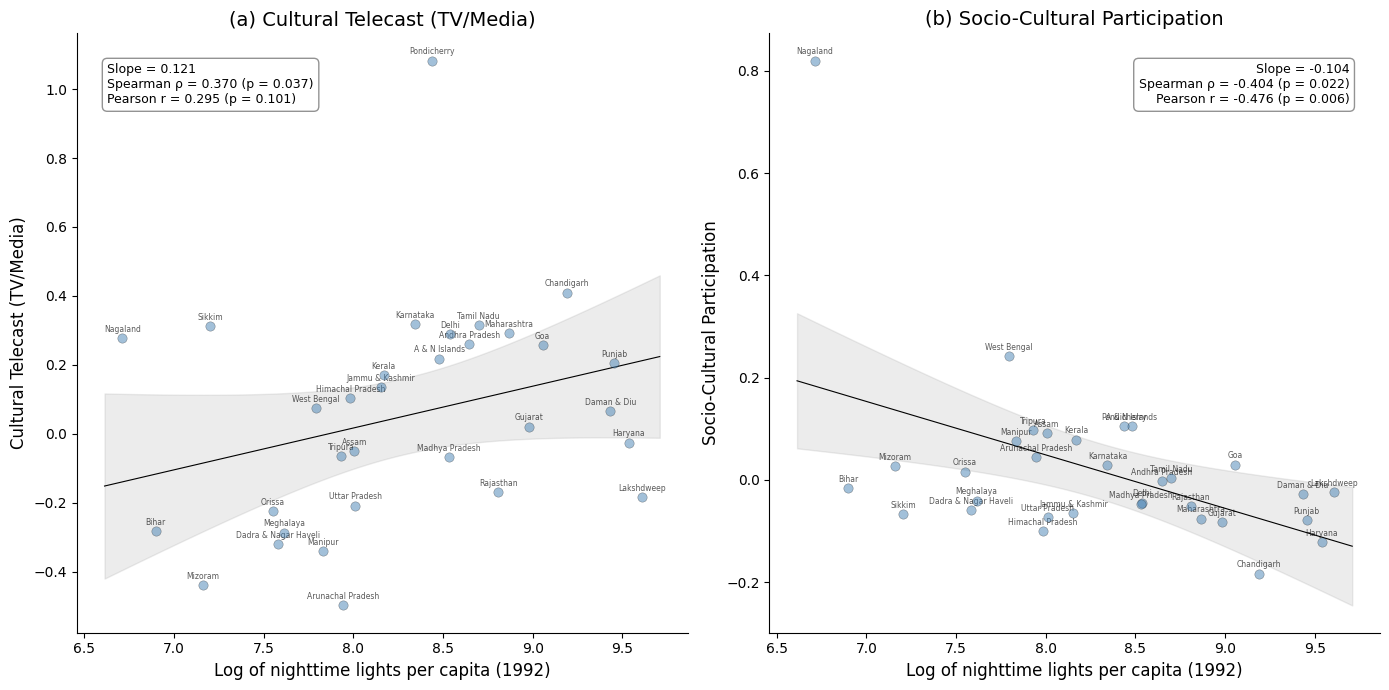
\includegraphics[keepaspectratio]{index_files/figure-latex/notebooks-c06_spatial_culture-fig-culture-scatter-output-1.png}}

}

\caption{\label{fig-culture-scatter}Relationship between nightlight
luminosity and cultural participation across 32 Indian states Notes:
Each point represents one of the 32 Indian states and union territories.
Panel (a) shows the bivariate relationship between log nighttime lights
per capita and cultural telecast (TV/media); Panel (b) shows the
relationship with socio-cultural participation. Solid line is the OLS
regression; gray band shows the 95\% confidence interval
(t-distribution, 30 df). Annotations report regression slope, Spearman
rank correlation, and Pearson correlation. Source: Nighttime lights from
CCNL DMSP-OLS (Zhao et al., 2022). Cultural participation from NSS 47th
Round (July--December 1991). See
\href{https://quarcs-lab.github.io/project2025s-py/notebooks/c06_spatial_culture.html}{Spatial
culture} notebook for source code.}

\end{figure}%

Cultural telecast (TV/media) exhibits a positive association with
nighttime light luminosity, with a Spearman rank correlation of 0.370
(\(p\) = 0.037). More luminous states therefore tend to rank higher on
the cultural telecast dimension.

In contrast, socio-cultural participation shows a significant negative
association, with a Spearman rank correlation of \$-\(0.404 (\)p\$ =
0.022). Less luminous states therefore tend to rank higher on
socio-cultural participation. This suggests that less urbanized regions
rely more on collective, in-person forms of cultural participation than
on media infrastructure.

Figure~\ref{fig-culture-lisa} presents the spatial distribution of these
two cultural variables through the lens of a LISA analysis. The low-low
cluster of cultural telecast in the northeast coincides with the low-low
cluster in the nighttime lights data, although the high-high clusters of
the two variables do not coincide. The significant high-high cluster in
cultural telecast is confined to the southern states, while the
northeastern states form a distinct high-high cluster in community-based
participation.

\begin{figure}[H]

\centering{

\pandocbounded{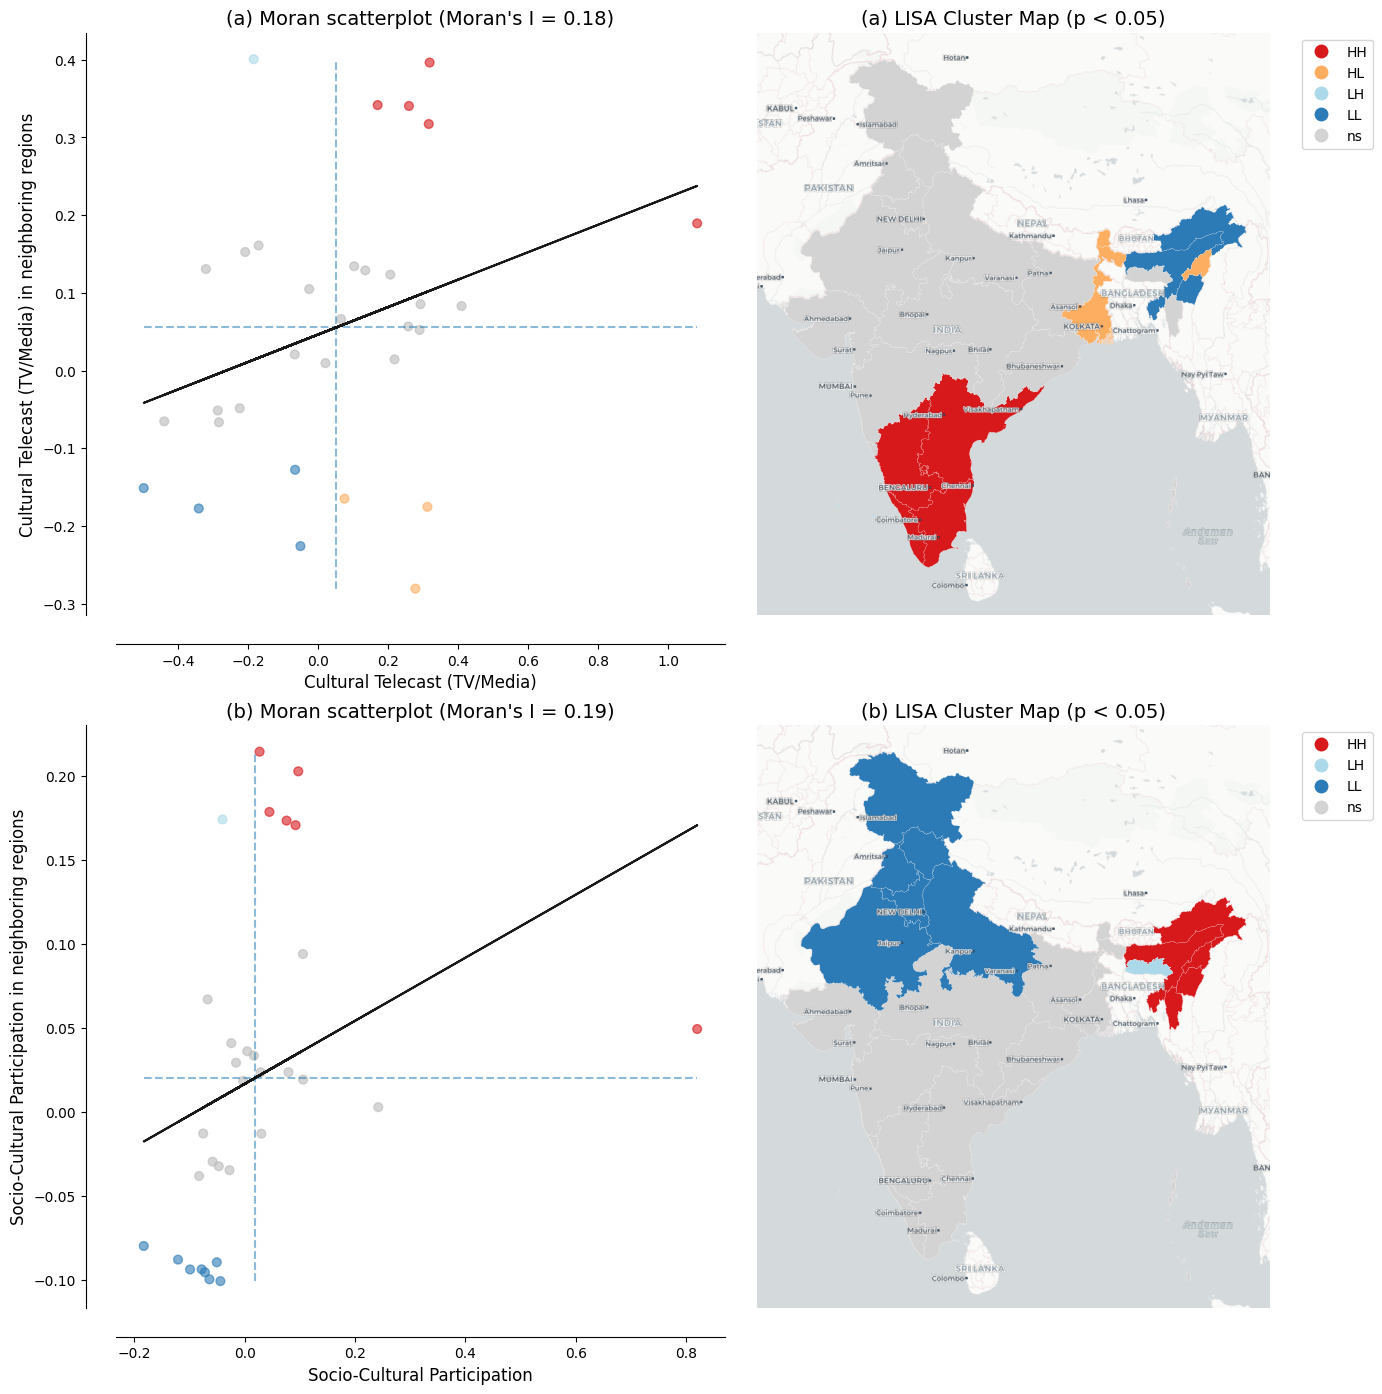
\includegraphics[keepaspectratio]{index_files/figure-latex/notebooks-c06_spatial_culture-fig-culture-lisa-output-1.png}}

}

\caption{\label{fig-culture-lisa}LISA cluster maps of cultural
participation across 32 Indian states Notes: Panel (a) shows results for
cultural telecast (TV/media); Panel (b) for socio-cultural
participation. Left subpanels show Moran scatterplots with the Global
Moran's I statistic. Right subpanels show LISA cluster maps with
statistically significant clusters at p \textless{} 0.05 based on 999
permutations and a 6-nearest-neighbors spatial weights matrix. Region
labels are overlaid from the CartoDB Positron basemap. Source: Cultural
participation data from NSS 47th Round (July--December 1991). See
\href{https://quarcs-lab.github.io/project2025s-py/notebooks/c06_spatial_culture.html}{Spatial
culture} notebook for source code.}

\end{figure}%

Together, the two correlations describe a pattern in which luminosity
ranks positively with media-based cultural participation and negatively
with community-based participation across states. The remaining four
cultural dimensions show no statistically significant association with
luminosity. These findings rest on a small cross-section of 32 states
observed at a single point in time, so larger datasets covering more
regions and periods would be needed to establish whether the patterns
are robust.

Two connections to the main analysis are worth drawing out, both offered
as interpretation rather than as findings. The first concerns what
luminosity measures. A positive association with media-based cultural
consumption and a negative one with community-based participation are
what one would expect if luminosity tracks electrification and
urbanization rather than economic output alone. The cultural results
are, in that sense, a small piece of evidence about the composite nature
of the proxy on which the convergence analysis rests, and they bear on
the measurement issues discussed below.

The second connection concerns spatial structure. Cultural participation
is not distributed randomly across states, since both dimensions
examined here are significantly spatially autocorrelated. Factors of
this kind, spatially clustered and correlated with development, are
precisely what a spatial Durbin model absorbs into its indirect effects
when they are not measured directly. We cannot test this with
state-level data for a single adjacent period, and we do not claim that
cultural participation drives the spillovers estimated in the results
section. What the exercise does is make concrete what a reduced-form
spatial model may be capturing, and it suggests that the Culture-Based
Development framework offers one route to testing the question directly,
should comparable data become available at the district level and over
time.

\subsection{New research directions}\label{new-research-directions}

Three kinds of gap limit what this literature can currently establish,
and each defines an agenda that the workflow used here is well placed to
support. The first two concern the raw material, namely the data
themselves and the geography those data cover. The third concerns the
range of theories those data have been used to test.

\subsubsection{Data gaps}\label{data-gaps}

Our analysis, following Chanda and Kabiraj (2020), relies on
radiance-calibrated DMSP-OLS nighttime lights for 1996 to 2010, a
dataset widely used as a proxy for economic activity (Henderson,
Storeygard, and Weil 2012; X. Chen and Nordhaus 2011). DMSP-OLS is
subject to well-documented limitations: top-coding in bright urban
cores, the absence of on-board calibration, and blooming artifacts that
spread light beyond its true source (Gibson et al. 2021; Abrahams, Oram,
and Lozano-Gracia 2018). These are not merely nuisances, and it is worth
being explicit about how they bear on our own estimates. Top-coding
compresses variation at the bright end of the distribution, which
affects the recorded initial luminosity of the most luminous districts.
Two opposing biases follow: classical measurement error in the regressor
attenuates the convergence coefficient toward zero, while measurement
error in initial luminosity that enters the growth rate with the
opposite sign works in the direction of overstating convergence. The net
effect is ambiguous in sign, and we do not claim to sign it. Measurement
error is also unlikely to be homogeneous across the sample, because the
association between luminosity and economic outcomes is stronger in
urban than in rural areas and Indian districts differ considerably in
how urbanized they are. Blooming has a clearer implication for the
spillover estimates that are central to this article. Because light
spills across district boundaries, part of what we measure as the
luminosity of a district originates with its neighbors, which
mechanically raises the apparent correlation between adjacent districts
and could therefore inflate the estimated indirect effects. That the
direct and total effects hold across all seven definitions of the
neighborhood, and the indirect effect under five of the seven
(Table~\ref{tbl-altw}), indicates they are not an artifact of any
particular neighbor definition, but it does not rule out blooming;
deblurring methods such as those of Abrahams, Oram, and Lozano-Gracia
(2018) offer one route to addressing it directly.

The Visible Infrared Imaging Radiometer Suite (VIIRS), operational since
2012, improves on DMSP-OLS in spatial resolution (roughly 750 meters
against 2.7 kilometers), in on-board radiometric calibration, and in
dynamic range, avoiding saturation in bright areas while detecting dim
lights in rural settlements (Elvidge et al. 2017; Gibson et al. 2021).
The discontinuity between the DMSP (1992--2013) and VIIRS
(2012--present) sensor eras remains an obstacle to long-run work, which
harmonization efforts have begun to address (Li et al. 2020), and recent
global series adjust explicitly for top-coding, blooming, and changes of
satellite system (Chiovelli et al. 2026). Beyond better sensors,
combining lights with other satellite products improves measurement
where lights alone are weak.\footnote{Lights have been combined with
  daytime imagery for poverty prediction (Jean et al. 2016), with land
  cover in agricultural areas (Keola, Andersson, and Hall 2015), with
  multiple remote sensing indicators for subnational output (Y. Chen,
  Ursavaş, and Mendez 2024; Suleiman, Nguyen, and Mendez 2025), and with
  survey data for multidimensional poverty (Khoun et al. 2025).}
Applying such multi-source approaches to Indian districts, and
re-estimating our specification on harmonized or VIIRS-era data, are the
most immediate extensions of the analysis reported here.

\subsubsection{Geographic gaps}\label{geographic-gaps}

A distinctive advantage of nighttime lights is that a single instrument
observes the entire planet under a common protocol, so that measurements
are comparable across countries and across regions in a way that
national accounts, compiled under different statistical systems and
capacities, are not (Henderson, Storeygard, and Weil 2012).
Comparability across settings and scales nevertheless requires explicit
adjustment (Chiovelli et al. 2026). This global coverage is, however,
coverage of light rather than of economic activity, and the distinction
determines where the method works. Roughly one fifth of the settlement
footprint of the planet emits no radiance detectable from space, and
unlit settlements are concentrated in Africa, which accounts for 39\% of
them, rising to 65\% when only rural settlement areas are considered
(McCallum et al. 2022). Lights therefore measure development that is
illuminated: they track urban areas as they expand, and rural areas as
lighting infrastructure reaches them, but they are close to silent where
neither is happening. The empirical record matches this
description.\footnote{Across 34 sub-Saharan African countries the
  association between harmonized luminosity and household wealth is
  pronounced in urban areas and considerably weaker in rural ones (Jhamb
  et al. 2025), and systematic assessments of which product to use, and
  where, reach similar conclusions (Gibson et al. 2021).}

The resulting gap is not simply that some regions have gone unstudied.
Regional inequality and convergence have been examined with luminosity
across 49 African countries (Kacou 2022), as they have across Chinese
provinces (Glawe and Mendez 2024), Indonesian districts (Miranti and
Mendez 2023), Thailand (Tipayalai and Mendez 2024), and Turkey (Ursavaş
and Mendez 2023). The gap is that the places where lights carry the
least information, rural and sparsely electrified areas, are the same
places where administrative statistics are weakest, which is precisely
where a satellite proxy would be most valuable. Closing it calls less
for further applications of the same proxy than for validation against
ground data in those settings, and for the complementary sensors and
multi-source methods described above.

\subsubsection{Theoretical gaps}\label{theoretical-gaps}

Our cross-sectional framework documents an average effect and its
spillover component, but not heterogeneity across the distribution. One
direction is distributional: methods designed for that purpose could
reveal whether Indian districts converge to a single steady state or
form distinct clubs, and combining them with spatial econometrics could
expose spatial poverty traps or growth poles that average estimates
render invisible (Rey and Montouri 1999).\footnote{The relevant tools
  are distribution dynamics (Quah 1996) and the regression-tree methods
  developed for identifying multiple growth regimes (Durlauf and Johnson
  1995).} A second concerns identification: our estimates capture
spillovers in reduced form without establishing whether they run through
infrastructure, migration, technology diffusion, or market access, and
quasi-experimental designs such as that of Asher and Novosad (2020)
offer a route to isolating them.

Beyond convergence, luminosity is now used to study city size and urban
growth (Ch, Martin, and Vargas 2021), electrification and the provision
of public goods (Min et al. 2013), and armed conflict (Witmer and
O'Loughlin 2011). As in the exploratory extension above, the same data
can be turned on socioeconomic dimensions that are not economic output
at all, such as the cultural participation theorized by Tubadji (2025).
A rapidly growing use is impact evaluation, in which lights measure the
local effect of a policy or a shock at fine spatial scales (Bluhm and
McCord 2022). Here the literature has established a caveat: lights
discriminate differences across places far better than changes over
time,\footnote{VIIRS predicts cross-sectional GDP better than
  time-series GDP (X. Chen and Nordhaus 2019), and in India the
  elasticity of lights with respect to local outcomes is far lower in
  the time series than in the cross-section (Asher et al. 2021). The
  relationship between lights and growth is also unstable across regions
  in both Brazil and India (Bickenbach et al. 2016).} and their
responsiveness to output varies with baseline income, density, and
sector (Bluhm and McCord 2022).\footnote{An evaluation may therefore
  fail to detect a real effect where lights react weakly, or attribute
  to a policy what is in fact heterogeneity in the relationship between
  light and output.} Evaluations over short horizons that rest on
luminosity therefore require validation against local ground data before
their estimates can be interpreted. The design used here, a
fourteen-year horizon, rests mostly on cross-sectional variation, which
is what lights currently support best.

Taken together, these three gaps describe a research agenda rather than
a list of caveats, and none of the work they imply requires starting
from scratch. The pipeline behind this article is public, documented,
and executable in a browser. A reader who wants to ask whether the
patterns documented here hold in another country, in a later period,
under a different definition of the neighborhood, or for an outcome
other than economic output can open the relevant notebook, substitute
their own data, and re-run it. The appearance of spatial dependence in
convergence processes across very different institutional settings also
suggests that the questions raised here are not specific to India. That
is the contribution we would most like this article to make: not an
estimate of how quickly Indian districts converged between 1996 and 2010
alone, but a working template that lowers the cost of asking the same
question elsewhere.

\subsection{Research reproducibility and open
science}\label{research-reproducibility-and-open-science}

The complexity of satellite-based economic research, which involves
multi-step processing pipelines, spatial econometric estimation, and
geographic visualization, makes reproducibility both challenging and
essential. As Donaldson and Storeygard (2016) note, methodological
choices in processing remotely sensed data, such as sensor
inter-calibration, can affect the empirical conclusions. The same
applies further down our own pipeline, at the construction of the
spatial weight matrix. Our own robustness analysis is a case in point:
the estimated convergence effects survive seven definitions of the
neighborhood, but that is something a reader can only confirm because
the code that produced each of them is available.

Open-source tools and cloud platforms are lowering the barriers to this
kind of verification. Cloud-based notebooks, such as those developed by
Patnaik and Mendez (2024) for processing nighttime lights data, remove
the need for specialized local software. The combination of open data,
version-controlled code, and cloud execution makes the full pipeline,
from satellite imagery to econometric results, verifiable and extensible
by the broader research community.

\section{Concluding remarks}\label{concluding-remarks}

This article re-examines the regional convergence hypothesis across
Indian districts using satellite nighttime light data, interactive
visualizations, and spatial econometric modeling. Building on the work
of Chanda and Kabiraj (2020), we developed an interactive web-based
visualization tool, and our spatial autocorrelation analyses indicate
that spatial dependence is a notable characteristic of both the
satellite data and the regional convergence process in India. Estimates
from our spatial Durbin model indicate that incorporating spatial
spillovers increases the estimated speed of regional convergence. The
total convergence effect in our fully specified model is approximately
51\% larger than conventional non-spatial estimates, and the implied
half-life of regional disparities falls from roughly 23 years to 13.
This finding suggests that in this setting non-spatial convergence
models understate the speed of regional convergence, although the
comparison with other regional literatures shows that the direction of
this adjustment is specific to the setting rather than general. If the
estimated indirect effects reflect genuine spillovers, place-based
development interventions would have broader impacts than conventional
estimates suggest, since their benefits would reach neighboring
districts as well as the districts they target. If instead they partly
reflect activity displaced across district boundaries, as the evaluation
literature on Indian place-based programs cautions, the same estimates
would overstate what those interventions add in aggregate.

Our results also demonstrate the usefulness of satellite nighttime
lights for studying economic dynamics in countries where subnational
data are scarce, infrequent, or unreliable. Conventional economic
statistics at the district level are often unavailable or inconsistent
across administrative boundaries, especially in large developing
economies. Radiance-calibrated nighttime light data allowed us to
analyze 520 Indian districts at a spatial granularity that would be
difficult to achieve with traditional national accounts. This
data-driven approach is potentially transferable to other data-poor
contexts across the developing world, and the ongoing transition from
DMSP-OLS to the higher-resolution VIIRS sensor should yield more precise
measurement of subnational economic activity in future studies.

This study also shows how reproducible open-science practices can
strengthen the credibility and reach of scientific research. The entire
analytical pipeline is documented in Jupyter notebooks written in
Python, and the results are embedded within the manuscript through the
Quarto publishing framework.\footnote{A single manuscript source
  generates multiple output formats. The HTML version allows readers to
  engage with interactive visualizations, inspect the code of the
  computational notebooks, and re-evaluate the results in light of their
  source code.} By hosting the complete codebase and data in a public
GitHub repository, and by making the Python notebooks executable in the
cloud through Google Colaboratory, we aim to encourage broader adoption
of reproducible open-science practices. Section 4 sets out where we
believe the most valuable work now lies, in better data, in the regions
this method currently serves least well, and in the questions beyond
convergence that it is able to address. The materials accompanying this
article are meant to make starting on any of them straightforward.

\section{Acknowledgments}\label{acknowledgments}

This research project was supported by JSPS KAKENHI Grant Number
24K04884. During the preparation of this manuscript, the authors
acknowledge the use of Claude Code (Anthropic) to assist with manuscript
editing, computational notebook development, and research infrastructure
setup. After using this AI tool, the authors reviewed the outputs,
confirmed their accuracy, and take full responsibility for the content
of this publication.

\section{Conflict of Interest}\label{conflict-of-interest}

The authors declare no conflict of interest.

\section{Data and Code Availability}\label{data-and-code-availability}

All data and computational code used in this study are available in the
project repository at
\url{https://github.com/quarcs-lab/project2025s-py}. The interactive
HTML version of this manuscript
(\url{https://quarcs-lab.github.io/project2025s-py/}) embeds the
computational notebooks, allowing readers to inspect the complete
analytical pipeline from raw data to published results. Every analytical
notebook can be executed in the cloud using Google Colaboratory without
any local software installation: readers open the notebook and run it,
and the empirical results, figures, and tables of this article are
regenerated from the raw data. The computational notebooks are
implemented entirely in Python. An earlier implementation of the same
analysis used R and Stata, and the present Python results reproduce it.
The AIC values differ by a few units because the two packages count
parameters differently: Stata treats the error variance of the spatial
model as a free parameter, and its information criterion for the
fixed-effects regressions uses the rank of the robust covariance matrix,
which two single-district states leave short by two. The interactive
Earth Engine application linked in the text is a convenience layer for
visualizing the underlying imagery; its source code is included in the
first notebook, and none of the results reported in this article depend
on it.

\phantomsection\label{refs}
\begin{CSLReferences}{1}{0}
\bibitem[\citeproctext]{ref-abrahams_etal_deblurring}
Abrahams, Alexei, Christopher Oram, and Nancy Lozano-Gracia. 2018.
{``Deblurring DMSP Nighttime Lights: A New Method Using Gaussian Filters
and Frequencies of Illumination.''} \emph{Remote Sensing of Environment}
210: 242--58. \url{https://doi.org/10.1016/j.rse.2018.03.018}.

\bibitem[\citeproctext]{ref-abreu_etal_meta_convergence}
Abreu, Maria, Henri L. F. de Groot, and Raymond J. G. M. Florax. 2005.
{``A Meta-Analysis of \(\beta\)-Convergence: The Legendary 2\%.''}
\emph{Journal of Economic Surveys} 19 (3): 389--420.
\url{https://doi.org/10.1111/j.0950-0804.2005.00253.x}.

\bibitem[\citeproctext]{ref-adhikari_dhital_decentralization}
Adhikari, Bibek, and Saroj Dhital. 2021. {``Decentralization and
Regional Convergence: Evidence from Night-Time Lights Data.''}
\emph{Economic Inquiry} 59 (3): 1066--88.
\url{https://doi.org/10.1111/ecin.12967}.

\bibitem[\citeproctext]{ref-allaire_quarto}
Allaire, J. J., Charles Teague, Carlos Scheidegger, Yihui Xie, and
Christophe Dervieux. 2024. {``Quarto.''} \url{https://quarto.org}.

\bibitem[\citeproctext]{ref-anselin_spatial_analysis}
Anselin, Luc. 1988. \emph{Spatial Econometrics: Methods and Models}.
Springer. \url{https://doi.org/10.1007/978-94-015-7799-1}.

\bibitem[\citeproctext]{ref-anselin_lisa}
---------. 1995. {``Local Indicators of Spatial Association---{LISA}.''}
\emph{Geographical Analysis} 27 (2): 93--115.
\url{https://doi.org/10.1111/j.1538-4632.1995.tb00338.x}.

\bibitem[\citeproctext]{ref-asher_shrug_india}
Asher, Sam, Tobias Lunt, Ryu Matsuura, and Paul Novosad. 2021.
{``Development Research at High Geographic Resolution: An Analysis of
Night-Lights, Firms, and Poverty in India Using the SHRUG Open Data
Platform.''} \emph{The World Bank Economic Review} 35 (4): 845--71.
\url{https://doi.org/10.1093/wber/lhab003}.

\bibitem[\citeproctext]{ref-asher_novosad_rural_roads}
Asher, Sam, and Paul Novosad. 2020. {``Rural Roads and Local Economic
Development.''} \emph{American Economic Review} 110 (3): 797--823.
\url{https://doi.org/10.1257/aer.20180268}.

\bibitem[\citeproctext]{ref-barro_convergence_modernisation}
Barro, Robert J. 2015. {``Convergence and Modernisation.''} \emph{The
Economic Journal} 125 (585): 911--42.
\url{https://doi.org/10.1111/ecoj.12247}.

\bibitem[\citeproctext]{ref-barro_sala_convergence}
Barro, Robert J., and Xavier Sala-i-Martin. 1992. {``Convergence.''}
\emph{Journal of Political Economy} 100 (2): 223--51.
\url{https://doi.org/10.1086/261816}.

\bibitem[\citeproctext]{ref-basher_etal_bangladesh_lights}
Basher, Syed Abul, Salim Rashid, and Mohammad Riad Uddin. 2023.
{``Regional Convergence in {Bangladesh} Using Night Lights.''}
\emph{Applied Economics Letters} 30 (18): 2581--88.
\url{https://doi.org/10.1080/13504851.2022.2099798}.

\bibitem[\citeproctext]{ref-beyer_jain_sinha_covid}
Beyer, Robert C. M., Tarun Jain, and Sonalika Sinha. 2023. {``Lights
Out? COVID-19 Containment Policies and Economic Activity.''}
\emph{Journal of Asian Economics} 85: 101589.
\url{https://doi.org/10.1016/j.asieco.2023.101589}.

\bibitem[\citeproctext]{ref-beyer_yamada_district_banks}
Beyer, Robert C. M., and Takahiro Yamada. 2020. {``District-Level
Convergence and Public Banks in {India}.''} SSRN Working Paper.
\url{https://doi.org/10.2139/ssrn.3818578}.

\bibitem[\citeproctext]{ref-bickenbach_regional_gdp}
Bickenbach, Frank, Eckhardt Bode, Peter Nunnenkamp, and Mareike Söder.
2016. {``Night Lights and Regional GDP.''} \emph{Review of World
Economics} 152 (2): 425--47.
\url{https://doi.org/10.1007/s10290-016-0246-0}.

\bibitem[\citeproctext]{ref-bluhm_mccord_small_geographies}
Bluhm, Richard, and Gordon C. McCord. 2022. {``What Can We Learn from
Nighttime Lights for Small Geographies? Measurement Errors and
Heterogeneous Elasticities.''} \emph{Remote Sensing} 14 (5): 1190.
\url{https://doi.org/10.3390/rs14051190}.

\bibitem[\citeproctext]{ref-carrington_jimenez_ecuador_lights}
Carrington, Sarah J., and Pablo Jiménez-Ayora. 2021. {``Shedding Light
on the Convergence Debate: Using Luminosity Data to Investigate Economic
Convergence in {Ecuador}.''} \emph{Review of Development Economics} 25
(1): 200--227. \url{https://doi.org/10.1111/rode.12712}.

\bibitem[\citeproctext]{ref-caselli_etal_convergence_debate}
Caselli, Francesco, Gerardo Esquivel, and Fernando Lefort. 1996.
{``Reopening the Convergence Debate: A New Look at Cross-Country Growth
Empirics.''} \emph{Journal of Economic Growth} 1 (3): 363--89.
\url{https://doi.org/10.1007/BF00141044}.

\bibitem[\citeproctext]{ref-ch_martin_vargas_city_size}
Ch, Rafael, Diego A. Martin, and Juan F. Vargas. 2021. {``Measuring the
Size and Growth of Cities Using Nighttime Light.''} \emph{Journal of
Urban Economics} 125: 103254.
\url{https://doi.org/10.1016/j.jue.2020.103254}.

\bibitem[\citeproctext]{ref-chakrabarty_mukherjee_covid_convergence}
Chakrabarty, Manisha, and Subhankar Mukherjee. 2022. {``Impact of
{COVID}-19 on Convergence in {Indian} Districts.''} \emph{Indian Growth
and Development Review} 15 (2-3): 198--209.
\url{https://doi.org/10.1108/igdr-11-2021-0152}.

\bibitem[\citeproctext]{ref-chakravarty_dehejia_gst}
Chakravarty, Praveen, and Vivek Dehejia. 2017. {``Will {GST} Exacerbate
Regional Divergence?''} \emph{Economic and Political Weekly} 52
(25--26): 97--102.
\url{https://www.epw.in/journal/2017/25-26/notes/will-gst-exacerbate-regional-divergence.html}.

\bibitem[\citeproctext]{ref-chanda_cook_demonetization}
Chanda, Areendam, and C. Justin Cook. 2022. {``Was {India's}
Demonetization Redistributive? {Insights} from Satellites and
Surveys.''} \emph{Journal of Macroeconomics} 73: 103438.
\url{https://doi.org/10.1016/j.jmacro.2022.103438}.

\bibitem[\citeproctext]{ref-chanda_kabiraj_district_convergence}
Chanda, Areendam, and Sujana Kabiraj. 2020. {``Shedding Light on
Regional Growth and Convergence in India.''} \emph{World Development}
133: 104961. \url{https://doi.org/10.1016/j.worlddev.2020.104961}.

\bibitem[\citeproctext]{ref-chen_etal_satellite_notebook}
Chen, Meixu, Dominik Fahrner, Daniel Arribas-Bel, and Francisco Rowe.
2020. {``A Reproducible Notebook to Acquire, Process and Analyse
Satellite Imagery: Exploring Long-Term Urban Changes.''} \emph{REGION} 7
(2): R15--46. \url{https://doi.org/10.18335/region.v7i2.295}.

\bibitem[\citeproctext]{ref-chen_nordhaus_luminosity_gdp}
Chen, Xi, and William D. Nordhaus. 2011. {``Using Luminosity Data as a
Proxy for Economic Statistics.''} \emph{Proceedings of the National
Academy of Sciences} 108 (21): 8589--94.
\url{https://doi.org/10.1073/pnas.1017031108}.

\bibitem[\citeproctext]{ref-chen_nordhaus_viirs_crosssection}
---------. 2019. {``VIIRS Nighttime Lights in the Estimation of
Cross-Sectional and Time-Series GDP.''} \emph{Remote Sensing} 11 (9):
1057. \url{https://doi.org/10.3390/rs11091057}.

\bibitem[\citeproctext]{ref-chen_etal_turkey_viirs}
Chen, Yilin, Uğur Ursavaş, and Carlos Mendez. 2024. {``Can
Higher-Quality Nighttime Lights Predict Sectoral {GDP} Across
Subnational Regions? {Urban} and Rural Luminosity Across Provinces in
{Türkiye}.''} \emph{Letters in Spatial and Resource Sciences} 17 (1):
12. \url{https://doi.org/10.1007/s12076-024-00375-x}.

\bibitem[\citeproctext]{ref-chiovelli_global_south}
Chiovelli, Giorgio, Stelios Michalopoulos, Elias Papaioannou, and Tanner
Regan. 2026. {``Illuminating the Global South.''} \emph{The Economic
Journal}. \url{https://doi.org/10.1093/ej/ueaf134}.

\bibitem[\citeproctext]{ref-cook_shah_nregs}
Cook, C. Justin, and Manisha Shah. 2022. {``Aggregate Effects from
Public Works: Evidence from India.''} \emph{Review of Economics and
Statistics} 104 (4): 797--806.
\url{https://doi.org/10.1162/rest_a_00993}.

\bibitem[\citeproctext]{ref-diop_africa_spillovers}
Diop, Samba. 2018. {``Convergence and Spillover Effects in {Africa}: A
Spatial Panel Data Approach.''} \emph{Journal of African Economies} 27
(3): 274--84. \url{https://doi.org/10.1093/jae/ejx027}.

\bibitem[\citeproctext]{ref-donaldson_storeygard_remotesensing}
Donaldson, Dave, and Adam Storeygard. 2016. {``The View from Above:
Applications of Satellite Data in Economics.''} \emph{Journal of
Economic Perspectives} 30 (4): 171--98.
\url{https://doi.org/10.1257/jep.30.4.171}.

\bibitem[\citeproctext]{ref-durlauf_johnson_convergence_clubs}
Durlauf, Steven N., and Paul A. Johnson. 1995. {``Multiple Regimes and
Cross-Country Growth Behaviour.''} \emph{Journal of Applied
Econometrics} 10 (4): 365--84.
\url{https://doi.org/10.1002/jae.3950100404}.

\bibitem[\citeproctext]{ref-elvidge_etal_viirs}
Elvidge, Christopher D., Kimberly E. Baugh, Mikhail Zhizhin, Feng-Chi
Hsu, and Tilottama Ghosh. 2017. {``VIIRS Night-Time Lights.''}
\emph{International Journal of Remote Sensing} 38 (21): 5860--79.
\url{https://doi.org/10.1080/01431161.2017.1342050}.

\bibitem[\citeproctext]{ref-ertur_koch_spatial_growth}
Ertur, Cem, and Wilfried Koch. 2007. {``Growth, Technological
Interdependence and Spatial Externalities: Theory and Evidence.''}
\emph{Journal of Applied Econometrics} 22 (6): 1033--62.
\url{https://doi.org/10.1002/jae.963}.

\bibitem[\citeproctext]{ref-fischer_spatial_mrw}
Fischer, Manfred M. 2011. {``A Spatial Mankiw-Romer-Weil Model: Theory
and Evidence.''} \emph{Annals of Regional Science} 47 (2): 419--36.
\url{https://doi.org/10.1007/s00168-010-0384-6}.

\bibitem[\citeproctext]{ref-gennaioli_etal_growth_regions}
Gennaioli, Nicola, Rafael La Porta, Florencio Lopez-de-Silanes, and
Andrei Shleifer. 2014. {``Growth in Regions.''} \emph{Journal of
Economic Growth} 19 (3): 259--309.
\url{https://doi.org/10.1007/s10887-014-9105-9}.

\bibitem[\citeproctext]{ref-gibson_etal_ntl_measurement}
Gibson, John, Susan Olivia, Geua Boe-Gibson, and Chao Li. 2021. {``Which
Night Lights Data Should We Use in Economics, and Where?''}
\emph{Journal of Development Economics} 149: 102602.
\url{https://doi.org/10.1016/j.jdeveco.2020.102602}.

\bibitem[\citeproctext]{ref-glawe_mendez_china_luminosity}
Glawe, Linda, and Carlos Mendez. 2024. {``Harmonized Luminosity and
Economic Activity Across Provinces in {China}: {Cross}-Sectional
Differences, Regional Time Series, and Inequality Dynamics.''}
\emph{Applied Economics} 57: 10677--93.
\url{https://doi.org/10.1080/00036846.2024.2439583}.

\bibitem[\citeproctext]{ref-gorelick_gee}
Gorelick, Noel, Matt Hancher, Mike Dixon, Simon Ilyushchenko, David
Thau, and Rebecca Moore. 2017. {``Google {E}arth {E}ngine:
Planetary-Scale Geospatial Analysis for Everyone.''} \emph{Remote
Sensing of Environment} 202: 18--27.
\url{https://doi.org/10.1016/j.rse.2017.06.031}.

\bibitem[\citeproctext]{ref-hasan_etal_backward_districts}
Hasan, Rana, Yi Jiang, and Radine Michelle Rafols. 2021. {``Place-Based
Preferential Tax Policy and Industrial Development: Evidence from
{India}'s Program on Industrially Backward Districts.''} \emph{Journal
of Development Economics} 150: 102621.
\url{https://doi.org/10.1016/j.jdeveco.2020.102621}.

\bibitem[\citeproctext]{ref-henderson_storeygard_weil_lights}
Henderson, J. Vernon, Adam Storeygard, and David N. Weil. 2012.
{``Measuring Economic Growth from Outer Space.''} \emph{American
Economic Review} 102 (2): 994--1028.
\url{https://doi.org/10.1257/aer.102.2.994}.

\bibitem[\citeproctext]{ref-isla_castillo_etal_eu_cohesion}
Isla-Castillo, Fernando, Anna Garashchuk, and Pablo Podadera-Rivera.
2024. {``Cross-Sectional and Spatial Panel Data Analysis of Territorial
Economic Cohesion in the {European Union} Regions Based on Convergence
Approach: From 2 to 8 Per Cent?''} \emph{Socio-Economic Planning
Sciences} 95: 102012. \url{https://doi.org/10.1016/j.seps.2024.102012}.

\bibitem[\citeproctext]{ref-jean_etal_poverty_prediction}
Jean, Neal, Marshall Burke, Michael Xie, W. Matthew Davis, David B.
Lobell, and Stefano Ermon. 2016. {``Combining Satellite Imagery and
Machine Learning to Predict Poverty.''} \emph{Science} 353 (6301):
790--94. \url{https://doi.org/10.1126/science.aaf7894}.

\bibitem[\citeproctext]{ref-jha_talathi_colonial_india}
Jha, Priyaranjan, and Karan Talathi. 2024. {``Impact of Colonial
Institutions on Economic Growth and Development in {India}: Evidence
from Night-Lights Data.''} \emph{Economic Development and Cultural
Change} 72 (4): 1653--1708. \url{https://doi.org/10.1086/725058}.

\bibitem[\citeproctext]{ref-jhamb_africa_nightlights}
Jhamb, Prachi, Susana Ferreira, Patrick Stephens, Mekala Sundaram, and
Jonathan Wilson. 2025. {``Shedding Light on Development: Leveraging the
New Nightlights Data to Measure Economic Progress.''} \emph{PLOS ONE} 20
(2): e0318482. \url{https://doi.org/10.1371/journal.pone.0318482}.

\bibitem[\citeproctext]{ref-kacou_africa_convergence}
Kacou, Kacou Yves Thierry. 2022. {``Interregional Inequality in Africa,
Convergence, and Multiple Equilibria: Evidence from Nighttime Light
Data.''} \emph{Review of Development Economics} 26 (2): 918--40.
\url{https://doi.org/10.1111/rode.12851}.

\bibitem[\citeproctext]{ref-keola_etal_lights_poverty}
Keola, Souknilanh, Magnus Andersson, and Ola Hall. 2015. {``Monitoring
Economic Development from Space: Using Nighttime Light and Land Cover
Data to Measure Economic Growth.''} \emph{World Development} 66:
322--34. \url{https://doi.org/10.1016/j.worlddev.2014.08.017}.

\bibitem[\citeproctext]{ref-theara_etal_cambodia_poverty}
Khoun, Theara, Ate Poortinga, Nyein Soe Thwal, Iván González de Alba,
Andrea McMahon, and Carlos Mendez. 2025. {``Mapping the Dimensions of
Poverty Through Big Data, Socioeconomic Surveys and Machine Learning in
{Cambodia}.''} \emph{Social Indicators Research} 180 (3): 1593--1618.
\url{https://doi.org/10.1007/s11205-025-03718-3}.

\bibitem[\citeproctext]{ref-kluyver_jupyter}
Kluyver, Thomas, Benjamin Ragan-Kelley, Fernando Pérez, Brian Granger,
Matthias Bussonnier, Jonathan Frederic, Kyle Kelley, et al. 2016.
{``Jupyter Notebooks---a Publishing Format for Reproducible
Computational Workflows.''} In \emph{Positioning and Power in Academic
Publishing: Players, Agents and Agendas}, 87--90. IOS Press.

\bibitem[\citeproctext]{ref-knuth_literate}
Knuth, Donald E. 1984. {``Literate Programming.''} \emph{The Computer
Journal} 27 (2): 97--111. \url{https://doi.org/10.1093/comjnl/27.2.97}.

\bibitem[\citeproctext]{ref-lesage_pace_spatial_econometrics}
LeSage, James P., and R. Kelley Pace. 2009. \emph{Introduction to
Spatial Econometrics}. {Chapman and Hall/CRC}.
\url{https://doi.org/10.1201/9781420064254}.

\bibitem[\citeproctext]{ref-lessmann_seidel_regional_inequality}
Lessmann, Christian, and André Seidel. 2017. {``Regional Inequality,
Convergence, and Its Determinants: A View from Outer Space.''}
\emph{European Economic Review} 92: 110--32.
\url{https://doi.org/10.1016/j.euroecorev.2016.11.009}.

\bibitem[\citeproctext]{ref-li_etal_harmonization}
Li, Xuecao, Yuyu Zhou, Min Zhao, and Xia Zhao. 2020. {``A Harmonized
Global Nighttime Light Dataset 1992--2018.''} \emph{Scientific Data} 7
(1): 168. \url{https://doi.org/10.1038/s41597-020-0510-y}.

\bibitem[\citeproctext]{ref-lolayekar_mukhopadhyay_india_spatial}
Lolayekar, Aparna P., and Pranab Mukhopadhyay. 2019. {``Spatial
Dependence and Regional Income Convergence in {India} (1981--2010).''}
\emph{GeoJournal} 84 (4): 851--64.
\url{https://doi.org/10.1007/s10708-018-9893-0}.

\bibitem[\citeproctext]{ref-mccallum_unlit_settlements}
McCallum, Ian, Christopher Conrad Maximillian Kyba, Juan Carlos Laso
Bayas, Elena Moltchanova, Matt Cooper, Jesus Crespo Cuaresma, Shonali
Pachauri, et al. 2022. {``Estimating Global Economic Well-Being with
Unlit Settlements.''} \emph{Nature Communications} 13 (1).
\url{https://doi.org/10.1038/s41467-022-30099-9}.

\bibitem[\citeproctext]{ref-mellander_etal_lights_gdp}
Mellander, Charlotta, José Lobo, Kevin Stolarick, and Zara Matheson.
2015. {``Night-Time Light Data: A Good Proxy Measure for Economic
Activity?''} \emph{PLOS ONE} 10 (10): e0139779.
\url{https://doi.org/10.1371/journal.pone.0139779}.

\bibitem[\citeproctext]{ref-min_etal_electrification}
Min, Brian, Kwawu Mensan Gaba, Ousmane Fall Sarr, and Alassane
Agalassou. 2013. {``Detection of Rural Electrification in Africa Using
DMSP-OLS Night Lights Imagery.''} \emph{International Journal of Remote
Sensing} 34 (22): 8118--41.
\url{https://doi.org/10.1080/01431161.2013.833358}.

\bibitem[\citeproctext]{ref-miranti_mendez_indonesia}
Miranti, Ragdad Cani, and Carlos Mendez. 2023. {``Social and Economic
Convergence Across Districts in {Indonesia}: {A} Spatial Econometric
Approach.''} \emph{Bulletin of Indonesian Economic Studies} 59 (3):
421--45. \url{https://doi.org/10.1080/00074918.2022.2071415}.

\bibitem[\citeproctext]{ref-moran_spatial_autocorrelation}
Moran, P. A. P. 1950. {``Notes on Continuous Stochastic Phenomena.''}
\emph{Biometrika} 37 (1/2): 17--23.
\url{https://doi.org/10.2307/2332142}.

\bibitem[\citeproctext]{ref-mendez_patnaik_notebook}
Patnaik, Ayush, and Carlos Mendez. 2024. {``Exploring Economic Activity
from Outer Space: A {Python} Notebook for Processing and Analyzing
Satellite Nighttime Lights.''} \emph{REGION} 11 (1): 79--109.
\url{https://doi.org/10.18335/region.v11i1.493}.

\bibitem[\citeproctext]{ref-peng_reproducible}
Peng, Roger D. 2011. {``Reproducible Research in Computational
Science.''} \emph{Science} 334 (6060): 1226--27.
\url{https://doi.org/10.1126/science.1213847}.

\bibitem[\citeproctext]{ref-pinkovskiy_salaimartin_lights_poverty}
Pinkovskiy, Maxim, and Xavier Sala-i-Martin. 2016. {``Lights, Camera,
Income! Illuminating the National Accounts-Household Surveys Debate.''}
\emph{Quarterly Journal of Economics} 131 (2): 579--631.
\url{https://doi.org/10.1093/qje/qjw003}.

\bibitem[\citeproctext]{ref-quah_twin_peaks}
Quah, Danny T. 1996. {``Twin Peaks: Growth and Convergence in Models of
Distribution Dynamics.''} \emph{The Economic Journal} 106 (437):
1045--55. \url{https://doi.org/10.2307/2235377}.

\bibitem[\citeproctext]{ref-rey_spatial_inequality}
Rey, Sergio J. 2025. {``Spatial Inequality.''} \emph{REGION} 12 (1):
19--45. \url{https://doi.org/10.18335/region.v12i1.563}.

\bibitem[\citeproctext]{ref-rey_spatial_dynamics}
Rey, Sergio J., and Brett D. Montouri. 1999. {``US Regional Income
Convergence: A Spatial Econometric Perspective.''} \emph{Regional
Studies} 33 (2): 143--56.
\url{https://doi.org/10.1080/00343409950122945}.

\bibitem[\citeproctext]{ref-rowe_etal_notebooks_region}
Rowe, Francisco, Gunther Maier, Daniel Arribas-Bel, and Sergio J. Rey.
2020. {``The Potential of Notebooks for Scientific Publication,
Reproducibility and Dissemination.''} \emph{REGION} 7 (3): E1--5.
\url{https://doi.org/10.18335/region.v7i3.357}.

\bibitem[\citeproctext]{ref-salaimartin_regional_cohesion}
Sala-i-Martin, Xavier X. 1996. {``Regional Cohesion: Evidence and
Theories of Regional Growth and Convergence.''} \emph{European Economic
Review} 40 (6): 1325--52.
\url{https://doi.org/10.1016/0014-2921(95)00029-1}.

\bibitem[\citeproctext]{ref-santos_marquez_etal_indonesia_spatial}
Santos-Marquez, Felipe, Anang Budi Gunawan, and Carlos Mendez. 2022.
{``Regional Income Disparities, Distributional Convergence, and Spatial
Effects: Evidence from {Indonesian} Regions 2010--2017.''}
\emph{GeoJournal} 87 (3): 2373--91.
\url{https://doi.org/10.1007/s10708-021-10377-7}.

\bibitem[\citeproctext]{ref-shenoy_place_based_policy}
Shenoy, Ajay. 2018. {``Regional Development Through Place-Based
Policies: Evidence from a Spatial Discontinuity.''} \emph{Journal of
Development Economics} 130: 173--89.
\url{https://doi.org/10.1016/j.jdeveco.2017.10.001}.

\bibitem[\citeproctext]{ref-solow_growth}
Solow, Robert M. 1956. {``A Contribution to the Theory of Economic
Growth.''} \emph{Quarterly Journal of Economics} 70 (1): 65--94.
\url{https://doi.org/10.2307/1884513}.

\bibitem[\citeproctext]{ref-hussein_etal_vietnam_ml}
Suleiman, Hussein, Minh-Thu Thi Nguyen, and Carlos Mendez. 2025.
{``Predicting Subnational {GDP} in {Vietnam} with Remote Sensing Data:
{A} Machine Learning Approach.''} \emph{Letters in Spatial and Resource
Sciences} 18 (1): 5. \url{https://doi.org/10.1007/s12076-025-00397-z}.

\bibitem[\citeproctext]{ref-tamiminia_gee_review}
Tamiminia, Haifa, Bahram Salehi, Masoud Mahdianpari, Lindi J.
Quackenbush, Sarina Adeli, and Brian Brisco. 2020. {``Google {E}arth
{E}ngine for Geo-Big Data Applications: A Meta-Analysis and Systematic
Review.''} \emph{ISPRS Journal of Photogrammetry and Remote Sensing}
164: 152--70. \url{https://doi.org/10.1016/j.isprsjprs.2020.04.001}.

\bibitem[\citeproctext]{ref-tipayalai_mendez_thailand}
Tipayalai, Katikar, and Carlos Mendez. 2024. {``Regional Convergence and
Spatial Dependence in {Thailand}: {Global} and Local Assessments.''}
\emph{Journal of the Asia Pacific Economy} 29 (2): 693--720.
\url{https://doi.org/10.1080/13547860.2022.2041286}.

\bibitem[\citeproctext]{ref-tubadji_cultural_entropy}
Tubadji, Annie. 2025. {``Cultural Entropy, Innovation, and Growth.''}
\emph{Politics \& Policy} 53 (4): e70050.
\url{https://doi.org/10.1111/polp.70050}.

\bibitem[\citeproctext]{ref-ursavas_mendez_turkey}
Ursavaş, Uğur, and Carlos Mendez. 2023. {``Regional Income Convergence
and Conditioning Factors in {Turkey}: {Revisiting} the Role of Spatial
Dependence and Neighbor Effects.''} \emph{Annals of Regional Science} 71
(2): 363--89. \url{https://doi.org/10.1007/s00168-022-01168-0}.

\bibitem[\citeproctext]{ref-witmer_lights_conflict}
Witmer, Frank D. W., and John O'Loughlin. 2011. {``Detecting the Effects
of Wars in the Caucasus Regions of Russia and Georgia Using
Radiometrically Normalized DMSP-OLS Nighttime Lights Imagery.''}
\emph{GIScience \& Remote Sensing} 48 (4): 478--500.
\url{https://doi.org/10.2747/1548-1603.48.4.478}.

\end{CSLReferences}




\end{document}
